\documentclass[paper=A4, 12pt, mathscr]{report}
\usepackage[top=0.9in, bottom=0.9in, left=0.7in, right=0.9in]{geometry}
\usepackage[none]{hyphenat}
\sloppy
\emergencystretch=3em
\usepackage{eucal, amssymb,amsmath,graphicx, amsfonts, latexsym}
\usepackage{algorithm}
\usepackage{algpseudocode}
\usepackage{color}
\usepackage{etoolbox}
\usepackage{mathtools}
\usepackage{listings}

%\renewcommand{\familydefault}{\ttdefault} %output font command sf rm tt
\renewcommand*\rmdefault{bch} %output font command- eg ppl cmr Imr pbk pnc ptm bch pag cmss Imss phv
\newcommand{\blue}[1]{\color{blue}#1}
\newenvironment{figurehere}
{\def\@captype{figure}}
\makeatother
\parindent 0pt
\definecolor{green}{rgb}{0,0.75,0}
\newcommand{\green}[1]{\color{green}#1}
\definecolor{orange}{rgb}{1,0.5,0}
\newcommand{\orange}[1]{\color{orange}#1}
\usepackage{xcolor}
\usepackage{float}
\usepackage[linktoc=page,colorlinks=true,linkcolor=black,citecolor=blue,urlcolor=blue]{hyperref}%cyan,magenta,red,brown,blue,green,yellow, %linktoc=all - toc page numbers with same color as toc entries...linktoc=black ...toc page numbers are black

\usepackage{tabularx}
\usepackage{hyperref}
\linespread{1.5}
\usepackage{enumerate}
\usepackage[title,toc,page]{appendix}

\usepackage[parfill]{parskip}
\usepackage{fancyhdr}
%\fancyhf{}
%\pagestyle{fancy}
\usepackage{afterpage}
\renewcommand{\headrulewidth}{1.2pt}
\renewcommand{\footrulewidth}{0pt}
\usepackage{pdfpages}
\usepackage{float,amsthm}
\usepackage{caption}
\usepackage{setspace}
\usepackage{tocloft}
\setlength{\cftbeforetoctitleskip}{-30pt}%space above toc
\setlength{\cftbeforeloftitleskip}{-30pt}%%space above lof
\setlength{\cftbeforelottitleskip}{-30pt}%space above lot
%\setcounter{tocdepth}{1}
%\renewcommand{\cftchapfont}{\normalfont} %No bold for toc entries
%\renewcommand{\cftchappagefont}{\normalfont}%No bold for items' page             
%#s in toc
\renewcommand{\cftsecleader}{\bfseries\cftdotfill{\cftsecdotsep}}% dots for sections only in toc
%\renewcommand{\cftchapleader}{\bfseries\cftdotfill{\cftsecdotsep}}%dots for all entries in toc
\usepackage{epsfig}
\usepackage{amsfonts}
\usepackage{tikz}
\usetikzlibrary{shapes.geometric, shapes.misc, arrows.meta, positioning}
\newcommand{\R}{\mathbb R}
\newcommand{\C}{\mathbb C}
\newtheorem{theorem}{Theorem}%[section]
\newtheorem{definition}{Definition}[section]
\newtheorem{lemma}{Lemma}%[section]
\newtheorem{remark}{Remark}%[section]
\newtheorem{corollary}{Corollary}%[section]
\newtheorem{proposition}{Proposition}%[section]
\def\E{{\mathcal E}}
%\usepackage{lineno}%package for adding line numbers
\renewcommand{\contentsname}{\centerline{\large TABLE OF CONTENTS}}% changing contents to table of contents
\renewcommand{\chaptername}{CHAPTER}

\renewcommand{\cftlottitlefont}{\hspace*{\fill}\large\bfseries}%Centering List of tables
\renewcommand{\cftafterlottitle}{\hspace*{\fill}}%Centering List of tables
\renewcommand{\cftloftitlefont}{\hspace*{\fill}\large\bfseries}%Centering List of figures
\renewcommand{\cftafterloftitle}{\hspace*{\fill}}%Centering List of figures
\usepackage{ctable}
\setlength{\parskip}{10pt}%space between paragraphs
\begin{document}
	\title{}
	\author{}
	%\baselineskip 22pt%distance between adjacent items in table of contents
	
	\makeatletter
	
	\def\@makechapterhead#1{%
		\begin{centering}
			{ \reset@font {\bf\large \scshape CHAPTER \thechapter}
				\par\nobreak\interlinepenalty\@M
				\large \bfseries #1\par\nobreak
				\vskip 10\p@}
		\end{centering}
	}
	\newpage
	
	\newpage
	\thispagestyle{empty}
	\begin{center}
		\begin{figure}
			\centering
			\includegraphics[width=30mm]{UnimaLogo.png}
		\end{figure}
		{\bf UNIVERSITY OF MALAWI\\
			\vskip 30pt
			MATHEMATICAL SCIENCES DEPARTMENT}
		\vskip 30pt
		{\bf SIMULTANEOUS ROUTING OF EMERGENCY VEHICLES IN CONGESTED URBAN NETWORKS}
		
		\vskip 30pt
		
		
		{\bf BY}\\
		{\bf {JOSOPHAT MAKAWA\\ 
				(BSC/MAT/14/21)}}
		
		\vskip 30pt
		
		{\bf SUPERVISOR}\\
		{\bf ASSOC. PROF. E. MWAKILAMA}
		
		\vskip 30pt
		
		{\bf A PROJECT SUBMITTED IN PARTIAL FULFILMENT OF THE\\ REQUIREMENTS FOR THE AWARD OF THE DEGREE OF\\ BACHELOR OF SCIENCE IN MATHEMATICS}
		
		\vskip 50pt
		
		{\bf MAY, 2026}
		
	\end{center}
	
	\newpage
	\begin{center}
		{\bf \large \scshape CERTIFICATION } \vskip 30pt
	\end{center}
	\addcontentsline{toc}{section}{Certification} The undersigned certify that they have read and hereby recommend for acceptance by the Mathematical Sciences Department at Chancellor College, the project titled: {\bf\emph{Simultaneous Routing of Emergency Vehicles in Poorly Developed and Congested Urban Networks}}, in partial fulfillment of the requirements for the award of the degree of Bachelor of Science/Education by the University of Malawi.
	
	\vskip 80pt
	
	%\begin{center}
	ASSOC. PROF. E. MWAKILAMA
	------------------------------------ \hfill {\bf Date:} --------------------------------------\\
	{\bf Name of Supervisor\\(Supervisor)}\\
	
	\ \\ 
	
	------------------------------------------------------ \hfill {\bf Date:} --------------------------------------\\
	{\bf Name of Supervisor\\(Supervisor)}\\
	
	%\end{center}
	
	\cfoot{\thepage}
	\pagenumbering{roman}
	\newpage
	\begin{center}
		{\bf \large \scshape  DECLARATION} \vskip 30pt
	\end{center}
	\addcontentsline{toc}{section}{Declaration}
	I, {\bf Josophat Makawa}, declare that this project is my own original work and that 
	it has not been presented and will not be presented to any other university for a similar or 
	any other degree award. Where somebody's work or results have been used, proper acknowledgements have been made.
	
	\vskip 150pt
	%\begin{center}
	Signed\\
	\vskip 7pt
	\rule{8cm}{0.3mm}\hfill {\bf Date:} \rule{5cm}{0.3mm}\\
	{\bf Full registered name of student}\\
	%\vskip 40pt
	%{\bf Signed\, ---------------------------------------\\
		%Full Name of Student}\\
	%\end{center}
	
	\newpage
	\begin{center}
		{\bf \large \scshape ACKNOWLEDGEMENT} \vskip 30pt
	\end{center}
	\addcontentsline{toc}{section}{Acknowledgement}
	I thank God for the beautiful life He has given me. I thank my parents, brother, and all relatives who have supported me in my studies from young age until now. Finally, I also thank my lecturers, and my friends for always being there when i pursued for the knowledge that led me here.
	\newpage
	\begin{center}
		{\bf \large \scshape DEDICATION} \vskip 30pt
	\end{center}
	\addcontentsline{toc}{section}{Dedication}
	\begin{center}
		To my parents and brother, whose sacrifices made every page of this work possible.
	\end{center}
	\newpage
	\begin{center}
		{\bf \large \scshape  ABSTRACT} \vskip 30pt
	\end{center}
	
	\addcontentsline{toc}{section}{Abstract}

	\newpage
	\setcounter{tocdepth}{2}
	\tableofcontents%\addcontentsline{toc}{section}{Table of Contents}
	\newpage
	\renewcommand*\listtablename{LIST OF TABLES}
	\listoftables \addcontentsline{toc}{section}{List of Tables}
	\newpage
	\renewcommand*\listfigurename{LIST OF FIGURES} 
	\listoffigures \addcontentsline{toc}{section}{List of Figures}
	\newpage
	\begin{center}
		{\bf\large \scshape LIST OF ABBREVIATIONS} \vskip 30pt
	\end{center}
	\addcontentsline{toc}{section}{List of Abbreviations}
	All abbreviations/acronyms (and their names) used in the project should be listed here. For example;\\
	
	\begin{tabular}{llllll}
		{\bf CBD}    &&&&& Central Business District\\
		{\bf EMV}    &&&&& Emergency Motor Vehicle\\
		{\bf FIFO}   &&&&& First-In-First-Out\\
		{\bf GIS}    &&&&& Geographic Information System\\
		{\bf GPS}    &&&&& Global Positioning System\\
		{\bf MOO}    &&&&& Multi-Objective Optimisation\\
		{\bf MOLS}   &&&&& Multi-Objective Label-Setting\\
		{\bf MWK}    &&&&& Malawian Kwacha\\
		{\bf OSM}    &&&&& OpenStreetMap\\
		{\bf VRP}    &&&&& Vehicle Routing Problem
	\end{tabular}
	
	\newpage
	\pagenumbering{arabic}
	\chapter{INTRODUCTION}
	\section{General Introduction}
	Emergency services such as ambulances, police, and fire brigades play a critical role in saving lives and protecting property. The effectiveness of these services largely relies on how fast and how reliably they can reach the affected areas \cite{10}. However, in most developing countries including Malawi, these services do not satisfy customer needs due to the nature of network infrastructure, poor connectivity, congestion and other factors. In Market areas, for example, congestion varies visibly with time of day. Thus, routes passing through market places can be optimal and the fastest at ones time but be non-optimal and the slowest during their respective market's peak hours.
	
	Traditional optimization methods that are mostly in use currently, focus on finding the fastest path. However, in practice, the fastest paths might not always be reliable or cost efficient. In addition, roads may become blocked, impassable and heavily congested which might lead to delays and increased fatality \cite{yan2021}. As such, recent research, has been focusing on finding fastest routes that are, at the same time, reliable and operationally cost effective. Such focus is widely known as the Multi-Objective Optimisation (MOO) \cite{tirkolaee2020}. On the converse, understanding points and path segments of great importance in a network whose closure or blockage can slow down the entire network is also very important \cite{luan2024}. According to Hao et al. \cite{hao2024}, determining these bottlenecks helps to understand network resilience which is the ability of the network to offer alternative routes under various ripple effects caused by these critical nodes.
	
	This study proposes the use of a simultaneous routing approach for emergency vehicles operating in a congested, poorly-planned urban road network characteristic of developing cities. Within this urban context, the model uses multi-objective optimization (MOO) to balance travel time, route reliability and operational cost \cite{tirkolaee2020,ding2021}, and couples this with a critical-analysis of the network to identify key nodes and intersections whose closure or severe congestion disproportionately affects overall network flow \cite{luan2024, hao2024, 6}. Because multiple emergencies may occur at the same time, the approach also explicitly considers multiple‐vehicle dispatching and routing, including emergency prioritisation \cite{7} and the simultaneous distribution of emergency vehicles to multiple incidents within the same network \cite{8}. The model is evaluated using synthetic data generated to reflect the road network characteristics of Zomba, Malawi---a representative developing-city context where observations of congestion patterns and infrastructure conditions informed parameter calibration, though all simulation data are synthetically generated for reproducibility and methodological generality. By capturing the realities of varying congestion patterns, dynamic infrastructure constraints and resource limitations typical of developing cities, the framework provides a better picture of how the network can handle multiple emergency response demands quickly and reliably.
	
	\section{Statement of the Problem}
	
	It has long been evident that urban road networks in most developing countries are insufficient, poorly planned, congested, and characterized by weak infrastructure  \cite{dumas2025, gonzalez2023}. These conditions are common for most developing countries worldwide and cause significant delays in emergency responses since travel time and route reliability are directly influenced by congestion and road quality \cite{9}. The situation becomes more critical during peak hours, especially around market areas, where roadside trading and human activity significantly reduce traffic flow capacity.
	
	Several studies have attempted to address emergency vehicle routing by focusing on shortest or fastest paths, assuming that travel times are constant and network conditions remain stable. For instance,  Amoako et al. \cite{10} and Yan et al. \cite{yan2021} proposed models that optimized emergency routes based on minimum travel time, but both assumed static traffic conditions, overlooking the impact of temporal congestion variations typical of developing cities. Similarly, Tirkolaee et al. \cite{tirkolaee2020} and Ding et al.\cite{ding2021} introduced multi-objective routing frameworks that considered travel cost and reliability but still failed to incorporate time-dependent congestion effects and dynamic road blockages. As a result, these models are less applicable in urban settings where congestion patterns vary hourly and can completely reverse optimal routes during market peaks.
	
	Moreover, most previous routing models treat each emergency independently and do not account for simultaneous incidents that compete for limited road resources and emergency vehicles. Researchers like Ganderi \cite{7} and Luan and Jiang \cite{luan2024} emphasized the importance of prioritization in emergency response but did not consider concurrent routing or how network disruptions propagate when multiple emergencies occur. Therefore, there remains a significant research gap in developing a simultaneous emergency vehicle routing model that incorporates multi-objective optimization (time, reliability, and operational cost) while analysing critical network points whose closure or congestion can hinder overall response. Such a model is crucial for understanding the resilience of urban road networks and improving the coordination of emergency services in real-world congested settings.
	
	\section{Research Objectives}
	\subsection{General Objective}
	The aim of this study is to develop a multi-objective model for simultaneous emergency vehicle routing in congested and poorly planned urban road networks.
	
	\subsection{Specific Objectives}
	The specific objectives of this study are to:
	\begin{enumerate}[(i)]
		\item Design a multi-objective optimization model that balances travel time, reliability, and operational cost.
		\item Analyse model efficacy under vulnerable road segments and intersections that strongly affect emergency response.
		\item Simulate simultaneous routing for multiple vehicles and emergencies using the proposed model.
		%\item Evaluate the proposed framework using real or simulated data from a case study area.
	\end{enumerate}
	
	\section{Justification of the Study}
	
	This study is justified by the need to improve emergency response efficiency in developing countries' congested and poorly planned urban areas, where delays often determine life or death outcomes. Existing models \cite{10,tirkolaee2020,yan2021,ding2021}, largely designed for well-developed transport systems, fail to capture the dynamic and uncertain nature of African urban road networks. By focusing on simultaneous routing, this research introduces a realistic representation of how multiple emergency incidents interact within a constrained network environment.
	
	Secondly, the study contributes to the growing literature on dynamic vehicle routing by integrating multi-objective optimization and network criticality analysis within a simultaneous dispatch framework which is the most under-explored area in low-income contexts. From a policy perspective, the study may create a foundation of an advanced model that can provide city planners, emergency service departments, and policymakers with data-driven insights to enhance urban transport resilience, emergency preparedness, and infrastructure upgrade and prioritization.
	
	Further, the developed model offers a foundation for practical application in the form of a decision-support software tool tailored for urban emergency services in Malawi. By linking real-time or near-real-time traffic and network condition inputs (e.g., via GIS/GPS) to the simultaneous routing framework, such a tool could assist dispatch centres in selecting routes that balance speed, reliability and cost under multiple incident demands. In addition, the inputs of this model can be parametrized by publicly available like OSM for any urban network. Although this study focuses on model development and case-study evaluation, it is designed with implementation feasibility in mind, thereby bridging the gap between theoretical research and operational practice in low-resource urban environments.
	% ============================================================
	% CHAPTER 2: LITERATURE REVIEW 
	% ============================================================
	
	\chapter{LITERATURE REVIEW}
	\label{ch:litreview}
	
	\section{Introduction}
	\label{sec:lit_intro}
	
	This chapter surveys the mathematical methods and empirical findings that
	frame the present study. The review moves from general optimisation theory
	to applications in emergency vehicle routing, and closes on the gap this
	research addresses. Coverage spans work published roughly between 2013 and
	2025, with priority given to studies that are either methodologically
	relevant to the multi-objective label-setting approach developed in
	Chapter~\ref{ch:methodology}, or empirically grounded in developing-country
	urban contexts. The goal is not to catalogue every technique in the
	literature, but to assess honestly what existing approaches can and cannot
	deliver in a poorly planned, data-scarce network such as those typical of
	sub-Saharan African cities.
	
	
	% ------------------------------------------------------------
	\section{Classical Optimisation Methods}
	\label{sec:lit_theory}
	% ------------------------------------------------------------
	
	The routing of vehicles through an urban road network can be stated as a
	constrained combinatorial optimisation problem on a directed graph
	$G=(V,E)$, where $V$ is the set of intersections and $E$ the set of road
	segments. Finding paths that minimise one or more cost objectives over this
	structure is, in general, the same problem once side constraints or multiple
	objectives are introduced. The literature responds to this complexity through
	three broad families of methods namely exact algorithms, classical heuristics, and
	metaheuristics. Each family makes a different trade-off between solution
	quality and computational cost, and the choice among them is not merely
	technical but deeply contextual.
	
	\textbf{Exact methods} for shortest-path and routing problems trace their
	foundations to Dijkstra's algorithm, which finds a provably optimal path
	from a source node to all other nodes in $O(|E|+|V|\log|V|)$ time using a
	priority-queue implementation \cite{hao2024}. The algorithm's optimality
	rests on two structural properties, non-negative arc weights and the
	First-In-First-Out (FIFO) condition, which requires that a vehicle departing
	node $i$ before another cannot arrive at any successor node $j$ later. FIFO
	is critical in time-dependent networks because it prevents a label at time
	$t$ from being dominated by a label at $t' > t$ in ways that would
	invalidate the greedy relaxation step. When travel time functions
	$\tau_{ij}(t)$ are piecewise-linear and FIFO holds, Dijkstra's logic extends
	cleanly to time-dependent networks with only modest modifications
	\cite{humagain}. The single-objective case is thus well-solved, such that, given
	adequate data, the algorithm guarantees optimality and runs efficiently even
	on networks of realistic urban scale.
	
	The more demanding problem is multi-objective routing, where decision-makers
	must simultaneously minimise travel time, cost, reliability, and network
	vulnerability. No single path minimises all objectives concurrently;
	instead, the goal is to find the Pareto-optimal set of paths, that is, paths
	not dominated by any other path on all objectives at once. Exact
	multi-objective label-setting algorithms (MOLS) extend Dijkstra's framework
	by maintaining a set of non-dominated labels at each node rather than a
	single scalar cost \cite{14,16}. A label
	$\mathbf{L}=(f_1', f_2, f_3)$ is retained only if no existing label at the
	same node is at least as good on every objective and strictly better on at
	least one. The algorithm terminates with a complete Pareto front, and its
	correctness follows directly from the FIFO property and the monotonicity of
	label extension. Tirkolaee et al.\ \cite{tirkolaee2020} found that exact
	label-setting methods outperformed metaheuristics on networks of fewer than
	200 nodes, which places typical secondary African cities well within the
	range where exact approaches are both tractable and superior.
	
	\textbf{Heuristics} offer faster computation by sacrificing the optimality
	guarantee. Constructive heuristics such as greedy insertion build feasible
	solutions step by step and work well when the objective function has a simple
	structure. Local-search procedures then improve an initial solution by
	systematically exploring neighbouring solutions. In practice, heuristics
	can find good solutions quickly, but their quality depends heavily on
	network structure, and there is no reliable way to know how far below
	optimal any given solution lies. This uncertainty matters in emergency
	routing, where the cost of a poor route is measured in minutes, not merely
	efficiency metrics.
	
	\textbf{Metaheuristics} generalise local search through high-level strategies
	that allow temporary deterioration of solution quality to escape local optima.
	Genetic Algorithms (GA) maintain a population of candidate solutions and
	apply crossover and mutation operators drawn from the analogy of biological
	evolution; extensions such as NSGA-II manage Pareto dominance across
	populations and are widely used for multi-objective vehicle routing
	\cite{tirkolaee2020}. Particle Swarm Optimisation (PSO) updates candidate
	solutions by interpolating between each particle's personal best and the
	swarm's global best, modelling collective social learning. Ant Colony
	Optimisation (ACO) uses probabilistic pheromone-trail deposition to direct
	search toward promising regions, exploiting the natural analogy with foragers
	on a graph \cite{ding2021}. More recent variants such as Harris Hawks
	Optimisation introduce fresh metaphors but share the same underlying
	exploration-exploitation mechanics \cite{hussein2023}. As Du and Yi
	\cite{du} note, the proliferation of metaphor-driven algorithms since the
	2010s has outpaced meaningful algorithmic novelty; most converge on similar
	solutions with similar computational cost once parameters are properly tuned.
	
	The critical limitation of all metaheuristic methods is the absence of any
	optimality guarantee. Performance is sensitive to parameter choices
	(population size, learning rates, pheromone evaporation coefficients) that
	must be calibrated through prior experimentation, which itself requires
	representative data. For a practitioner in a resource-constrained setting
	who needs reliable routes when a patient is already in crisis, deploying a
	tuning-sensitive algorithm without strong empirical calibration is a risk
	the literature does not adequately acknowledge.
	
	Reinforcement learning (RL) represents a fourth paradigm, distinct from the
	three above in that it learns a routing policy through interaction with an
	environment rather than solving a fixed problem instance. Deep Q-Networks
	and multi-agent variants have achieved impressive results in simulation, but
	they require extensive offline training, GPU infrastructure, and environments
	that closely match deployment conditions \cite{yan2021, su2025}. The
	resulting policies are also difficult to inspect or audit, which is a
	practical concern for life-critical applications.
	
	In summary, exact label-setting methods provide the strongest theoretical
	foundation for multi-objective emergency routing in small-to-medium networks
	where optimality matters and data infrastructure is limited. Metaheuristics
	scale better but cannot guarantee solution quality. Reinforcement learning
	methods can adapt dynamically but impose data and computational requirements
	that are out of reach for most developing-country cities. This hierarchy of
	trade-offs determines what is and is not feasible for Zomba-scale networks.
	
	
	% ------------------------------------------------------------
	\section{Review of Related Studies}
	\label{sec:lit_related}
	% ------------------------------------------------------------
	
	The broad theoretical backdrop described above becomes much sharper when one
	looks at how these methods have been applied to actual emergency routing
	problems, and in particular at the contexts for which they were designed.
	
	\subsection*{Static and Single-Objective Approaches}
	
	The early emergency routing literature took static network conditions as
	given and optimised for a single objective, most often minimum travel time.
	Ogunwolu et al.\ \cite{15} applied Dijkstra's algorithm with historical
	traffic-speed adjustments to emergency response in Nigeria, reporting 18\%
	reductions in response time compared to experience-based driver routing.
	The result was practically meaningful, but the study acknowledged
	performance degraded substantially during unplanned congestion that fell
	outside the historical data. In effect, the model worked when reality matched
	its assumptions, which is precisely when routing optimisation matters least.
	Amoako \cite{10} reached similar conclusions in Kumasi, Ghana, noting that
	shortest-path algorithms repeatedly directed vehicles across bridges that
	were theoretically fast but practically unreliable under market-day
	congestion. The shortest route and the best route were not the same thing,
	and the gap between them widened exactly when demand was highest.
	
	These early findings established what the field's subsequent evolution
	confirms at every scale, that is, static assumptions are not a simplification, they
	are an error whose cost grows with network volatility.
	
	\subsection*{Dynamic and Learning-Based Methods}
	
	Recognising this, Yan et al.\ \cite{yan2021} developed a Prioritised
	Experience Replay Deep Q-Network (PERDQN) for ambulance routing on congested
	urban arterial roads, achieving a 67.1\% reduction in arrival time relative
	to the static shortest-path baseline. The result is striking. Yet the
	model required 10,000 training episodes with continuous sensor feeds and
	GPU computing resources to reach convergence, and it transferred poorly
	to network topologies not represented in training. Su \cite{su2025} extended
	this to a multi-agent setting where vehicles learn to coordinate, adding a
	further 23\% improvement at still higher computational cost. Alruwaili et
	al.\ \cite{alruwaili2025} combined LSTM networks with ResNet18 architectures
	for integrated routing and signal control, reporting 71.3\% response time
	reductions in simulation.
	
	Selvan et al.\ \cite{selvan2025} reduced training cost through transfer
	learning, cutting required episodes to approximately 5,000, while Jose and
	Grace \cite{jose2020} used evolutionary intelligence to achieve 43\%
	improvement in only 500 iterations. In both cases, however, the reduction in
	training cost did not eliminate the underlying data requirement, thus, historical
	traffic patterns are needed to construct the training environment, and
	those patterns are exactly what poorly-developed city networks rarely have.
	Building on these, Chowdhury et al.\ \cite{chowdhury2023} and Rezaee et
	al.\ \cite{rezaee2023} went further, adding IoT vehicle-to-infrastructure
	communication and UAV aerial surveillance to the pipeline. The resulting
	systems are impressive demonstrations of what is technically possible. They
	are also essentially undeployable in any city that does not already have
	reliable electricity, maintained sensor infrastructure, and institutional
	capacity to operate cloud computing systems.
	
	This progression reveals that the
	cities that most urgently need better emergency routing are the least equipped
	to deploy the algorithms that perform best. Improving performance on
	well-instrumented test networks in developed countries does not close the
	gap; it widens it.
	
	\subsection*{Multi-Objective Formulations}
	
	A parallel and more directly relevant body of work moves beyond single-objective
	minimisation. Sun et al.\ \cite{6} developed optimal reliable path algorithms
	that balance expected travel time against route variance, demonstrating that
	paths avoiding high-variability links were only 8--12\% longer in expectation
	but showed 40\% better reliability under congestion fluctuations. Their
	travel-time variability measure $\displaystyle v_{ij}(t) = \tau_{ij}(t) \cdot
	(\tau_{ij}(t)/\tau_{ij}^0)^2 \cdot \gamma$ explicitly penalises congested
	links, and the formulation is analytically tractable under FIFO
	piecewise-linear travel functions, making it a natural building block for
	multi-objective label-setting. Building on this, Zhao et al.\ \cite{16}
	added a safety objective in earthquake response scenarios, while Ding et
	al.\ \cite{ding2021} applied a hybrid PSO-ACO formulation to multi-depot
	relief logistics, achieving 18\% better objective values than either
	algorithm individually and demonstrating the importance of equity across
	affected areas through Gini-coefficient constraints \cite{liu2022epidemic}.
	
	Tirkolaee et al.\ \cite{tirkolaee2020} provide perhaps the most methodologically
	precise comparison in the multi-objective VRP literature. Their study of the
	reliable pollution-routing problem uses Pareto-based algorithms alongside
	exact methods and finds that exact label-setting consistently outperformed
	metaheuristics on instances with fewer than 200 nodes, with performance parity
	only appearing at larger scales. This finding reframes the default assumption
	that metaheuristics are the natural choice for multi-objective VRPs; for
	developing-country cities, where networks are typically in the 100--200 node
	range, exact methods may offer better results with comparable computation.
	
	In contrast to these methodological advances, the multi-objective literature
	shares a common structural weakness that travel time functions are typically
	assumed independent of departure time, network criticality is not modelled,
	and study settings are almost uniformly in well-developed urban environments
	with complete and accurate road network data.
	
	\subsection*{Network Criticality and Structural Vulnerability}
	
	An emerging body of work examines the structural properties of road networks
	themselves, asking which edges or nodes are most critical to overall
	connectivity. Sun et al.\ \cite{6} employ edge betweenness centrality, which
	measures the fraction of shortest paths in a network that pass through a
	given edge, to identify segments whose loss disproportionately degrades
	network flow. Kozhabek and Chai \cite{11} validate this approach across 25
	cities in a robustness analysis and found that grid-planned
	cities such as Chicago and Barcelona maintained roughly 80\% network
	efficiency after 40\% of edges were removed, while organically developed
	cities including Cairo, Mumbai, and Nairobi collapsed to 20\% efficiency
	after losing only 15\% of edges. That three-to-five-fold gap in structural
	vulnerability is not a marginal difference; it means that the same congestion
	event that causes minor delays in a planned grid can paralyse an organic
	network.
	
	Zainal et al.\ \cite{zainal2022} documented that a single bridge
	collapse in Jakarta rendered 37\% of the fire service's coverage area
	unreachable. Amoako's earlier Kumasi observations are displayed similar outcomes that high-centrality
	crossings were systematically avoided by experienced drivers even when they
	appeared optimal under the model. What these studies collectively establish
	is that criticality is not abstract topology, it translates to operational
	failures under the congestion conditions prevalent in developing-country
	networks. However, a gap remains. Neither Sun et al.\ \cite{6} nor Kozhabek
	and Chai \cite{11} integrated their criticality metrics into routing
	optimisation algorithms. The vulnerability is documented; it is not yet
	routinely avoided.
	
	\subsection*{Multi-Vehicle Coordination}
	
	Most routing literature routes a single vehicle to a single incident. Real
	emergency operations are more complicated in the sense that multiple incidents occur
	simultaneously, and a limited fleet must be allocated across them with
	consideration for congestion compounding as several vehicles traverse
	overlapping road segments at once.
	
	Li et al.\ \cite{12} addressed this through a sequential priority-based
	decomposition for freeway emergency response where vehicles are dispatched
	iteratively in priority order, with network state updated between dispatches
	to account for the congestion each vehicle introduces. Their method achieves
	approximately 95\% of optimal joint-routing solution quality while computing
	40\% faster, with a theoretical approximation error that shrinks
	counter-intuitively as fleet size grows, bounded by $\varepsilon(K) =
	O(1/\sqrt{K})$. Li et al.\ \cite{14} extended this framework to disaster
	scenarios with dynamic road damage updates, demonstrating 28\% improvement
	over static dispatch plans. Ghaderi and Momeni \cite{7} introduced explicit
	priority-based assignment, showing through facility location analysis that
	cardiac emergencies justify different vehicle allocation strategies than
	routine transports, and that ignoring priority degrades expected outcomes
	for the most severe cases.
	
	These results establish that sequential priority decomposition is both
	theoretically justified and practically tractable. However, all three studies
	assumed either freeway networks with high structural redundancy \cite{12}
	or well-documented disaster scenarios where road damage patterns are known in
	advance \cite{14}. Neither condition holds in an organic urban network where
	the primary routing challenge comes from unpredictable everyday congestion,
	limited path redundancy, and high criticality concentration in a small number
	of bridges or market-road intersections. In such networks, the assumption that
	vehicle interactions are primarily local, which underlies the decomposition
	approach's efficiency, may fail since a single congested bridge can force
	fleet-wide re-routing, turning what should be a local interaction into a
	global one.
	
	\subsection*{The Developing-Country Context}
	
	The final and most directly relevant strand of the literature examines
	emergency routing in cities where infrastructure is weak and data is scarce.
	Kalonde et al.\ \cite{9} conducted a systematic study of travel times in
	Blantyre, Malawi, with findings that deserve to be read carefully by anyone
	building routing models for African cities. OpenStreetMap coverage was 23\%
	incomplete, with roads used regularly by GPS-tracked vehicles missing from
	the database entirely. Identical journeys took 25 minutes in the dry season
	and 45 minutes in the rainy season. Market-area congestion added 40--60\%
	to travel times on affected corridors. Settlements within five kilometres of
	health facilities took over 90 minutes to reach by vehicle. These are not
	edge cases; they are the normal operating conditions.
	
	Mwakilama and Eneya \cite{8} documented comparable conditions in Zomba
	specifically, finding a 47\% gap between theoretically optimal routes derived
	from a transport optimisation model and the practically efficient routes
	developed by experienced drivers through trial and error. Market-day
	congestion, seasonal flooding on low-lying roads, and informal roadside
	commercial activity created routing conditions that the model could not
	capture because they were not encoded in the network data. Gonzalez-Navarro
	et al.\ \cite{gonzalez2023} generalise this pattern across developing
	countries, arguing that infrastructure heterogeneity, dramatic variation in
	road quality, accessibility, and reliability within the same city, demands
	context-sensitive modelling that generic optimisation frameworks are not
	designed to provide.
	
	Together, these studies establish that the problem this thesis addresses is
	not a harder version of the urban routing problem studied in the mainstream
	literature. It is a structurally different problem. The assumptions that most
	routing models treat as background conditions, complete and accurate network
	maps, predictable congestion patterns, stable road quality, available sensor
	data, are themselves the first things that fail in a city like Zomba.
	
	
	% ------------------------------------------------------------
	\section{Research Gap}
	\label{sec:lit_gap}
	% ------------------------------------------------------------
	
	Reading across the five strands reviewed above, the literature has produced
	three distinct bodies of work that have not yet been joined. Multi-objective
	routing methods (Sun et al.\ \cite{6}, Tirkolaee et al.\ \cite{tirkolaee2020},
	Ding et al.\ \cite{ding2021}) have formalised reliable Pareto-optimal path
	selection but have done so under time-independent travel costs or without
	any account of structural network vulnerability. Network criticality research
	(Kozhabek and Chai \cite{11}, Sun et al.\ \cite{6}) has produced rigorous
	characterisations of edge betweenness and vulnerability but has not
	translated these into routing algorithms that actively avoid high-criticality
	paths. Multi-vehicle coordination work (Li et al.\ \cite{12,14}, Ghaderi
	and Momeni \cite{7}) has established theoretically sound sequential
	decomposition frameworks but has tested them only on freeway networks or
	structured disaster scenarios with data and redundancy that organic
	developing-city networks do not have.
	
	The capability-need mismatch compounds this fragmentation. Methods that perform
	best in simulation, deep reinforcement learning, multi-agent RL,
	IoT-integrated systems, require training data volumes, sensor infrastructure,
	and computing resources that are inversely correlated with problem severity.
	Hao et al.\ \cite{hao2024} reviewed 78 emergency routing studies and found
	fewer than 6\% considered African contexts. Humagain et al.\ \cite{humagain2019}
	found the same pattern in a systematic review of 40 route optimisation
	papers, 89\% focused on developed-country cities. This is not merely an
	application gap that could be filled by transferring methods across contexts.
	The core assumptions built into the methods, rich real-time data, reliable
	infrastructure, well-mapped networks, do not hold where the routing problem
	is most acute.
	
	No existing framework simultaneously integrates; (i) a three-objective
	routing formulation balancing travel time, reliability, and network-structural
	resilience via edge betweenness centrality; (ii) coordinated multi-vehicle
	dispatch with sequential priority-based congestion interaction; and (iii)
	operation under the data-scarcity and infrastructure constraints typical of
	poorly developed organic urban networks. The intersection of these three
	requirements defines the gap this study fills. It is not enough to apply
	an existing method to a new geography; the method itself must be designed
	for a setting where the data infrastructure assumed by almost all prior
	work is unavailable.
	
	
	% ------------------------------------------------------------
	\section{Scope of the Study}
	\label{sec:lit_scope}
	% ------------------------------------------------------------
	
	This study focuses specifically on the multi-objective simultaneous routing
	of emergency vehicles in organic urban road networks with characteristics
	matching those documented for Zomba and Blantyre including, incomplete OSM data,
	time-dependent market-area congestion, high structural vulnerability in
	low-redundancy corridors, and the absence of real-time sensor infrastructure.
	The framework developed here minimises three objectives, the composite
	travel-time and cost objective $f_1'$, the route-reliability objective $f_2$,
	and the network-resilience objective $f_3$ based on edge betweenness
	centrality, using a Multi-Objective Label-Setting (MOLS) algorithm that
	operates within FIFO piecewise-linear travel time functions, requires no
	sensor data beyond a static or semi-static road network description, and
	remains computationally tractable on networks of the size typical of
	secondary African cities.
	
	Multi-vehicle dispatch is handled through a sequential priority-based scheme
	that updates network congestion state between dispatches, capturing the
	compounding delay effects when several vehicles operate simultaneously in
	a low-redundancy network. The framework is evaluated on a synthetic network
	of 40 nodes and 200 directed edges, parametrised to reflect the road-type
	speed profiles, market-peak congestion multipliers, and seasonal reliability
	characteristics documented in the Malawian routing literature \cite{8,9}.
	The study does not pursue real-time adaptive re-routing, nor does it model
	heterogeneous fleets; these are recognised limitations and directions for
	future work. The boundary is drawn at a framework that is both theoretically
	principled and deployable under resource constraints that the existing
	literature has largely treated as an afterthought.
	
	% ================================================================
	% CHAPTER 3: METHODOLOGY
	% ================================================================
	
	% ================================================================
	% CHAPTER 3: METHODOLOGY
	% ================================================================
	
	\chapter{METHODOLOGY}
	\label{ch:methodology}
	
	\section{Network Representation and Time-Dependent Travel Times}
	
	The urban road network is modelled as a directed graph $G=(V, E)$,
	where $V$ represents intersections, hospitals, and market areas, and $E$
	represents directed road segments. Each edge $(i,j) \in E$ carries a
	\textbf{time-dependent travel time function} $\tau_{ij}(t)$, giving the
	travel duration when departing node $i$ at time $t$
	\cite{yan2021,13,humagain}.
	
	We adopt the First-In-First-Out (FIFO) property throughout: if vehicle
	$A$ departs node $i$ before vehicle $B$, then $A$ arrives at node $j$ no
	later than $B$. While FIFO may be violated on heavily congested two-lane
	roads where overtaking occurs, we retain it as a necessary simplification
	for algorithmic tractability \cite{14,16,humagain}. The property ensures
	causality in the time-dependent network model: a routing decision made
	after a vehicle has entered a link cannot retroactively reduce that
	vehicle's travel time, so a later departure can never produce an earlier
	arrival \cite{14}.
	
	For ordinary road segments, $\tau_{ij}(t)$ is defined as a
	piecewise-linear function over four daily intervals
	\cite{13,humagain}:
	\begin{equation}
		\tau_{ij}(t)=
		\begin{cases}
			\tau_{ij}^0, & t\in[0,t_1) \\[2pt]
			\tau_{ij}^0 + s_{ij}^{\mathrm{am}}(t-t_1), & t\in[t_1,t_2) \\[2pt]
			\tau_{ij}^{\mathrm{peak}}, & t\in[t_2,t_3) \\[2pt]
			\tau_{ij}^{\mathrm{peak}} - s_{ij}^{\mathrm{pm}}(t-t_3),
			& t\in[t_3,t_4)
		\end{cases}
		\label{eq:tauij}
	\end{equation}
	where $\tau_{ij}^0 = \ell_{ij}/s_{ij}^0$ is the free-flow travel time,
	$\ell_{ij}$ is edge length, $s_{ij}^0$ is free-flow speed, and
	$s_{ij}^{\mathrm{am}}$, $s_{ij}^{\mathrm{pm}}$ are linear slopes
	describing morning build-up and evening dissipation. The intervals
	$[t_1,t_2)$ and $[t_3,t_4)$ correspond to morning and evening rush
	periods respectively \cite{13}.
	
	\subsection*{Highway Upgrade Classification and the Braess Paradox}
	
	A characteristic feature of poorly developed African cities such as Zomba
	is that road investment is spatially uneven: individual corridors are
	upgraded to trunk or dual-carriageway standard while the surrounding
	network remains unchanged. This pattern creates conditions that are
	theoretically described by Braess's paradox \cite{braess1968}, which
	demonstrates that adding capacity to a congested network can, under
	user-equilibrium routing, \textit{increase} total travel time across all
	users. The mechanism is indirect: the new high-capacity corridor attracts
	diverted traffic, which concentrates demand on the feeder roads that
	channel vehicles into it. The highway itself flows freely; its connectors
	become the new structural bottleneck. For emergency vehicles, the
	consequence is that routes traversing feeder segments adjacent to recently
	upgraded corridors become systematically less reliable as a downstream
	effect of an improvement elsewhere in the network, not because their own
	physical condition has deteriorated.
	
	To capture this formally, we partition $E$ into three disjoint classes:
	\begin{align}
		E_H &= \{\,(i,j)\in E : \text{trunk/highway segment}\,\},
		\nonumber\\
		E_F &= \{\,(i,j)\in E\setminus E_H :
		i\in\mathcal{N}_H \;\text{or}\; j\in\mathcal{N}_H\,\},
		\nonumber\\
		E_S &= E\setminus(E_H\cup E_F),
		\nonumber
	\end{align}
	where $\mathcal{N}_H$ denotes the set of nodes directly incident to at
	least one highway edge. Edges in $E_F$ are \textit{feeder} segments;
	all remaining edges belong to $E_S$.
	
	In secondary African cities, traffic volumes rarely approach highway
	saturation capacity \cite{gonzalez2023}. Highway edges are therefore
	assigned a time-invariant travel time:
	\begin{equation}
		\tau_{ij}(t) = \tau_{ij}^{0} = \frac{\ell_{ij}}{s_{ij}^{0}},
		\qquad \forall\,(i,j)\in E_H,\quad \forall\,t.
		\label{eq:hw_const}
	\end{equation}
	This is implemented by setting the congestion multiplier to $1.0$ across
	all time periods for $E_H$ edges, leaving the piecewise-linear structure
	of Eq.~\eqref{eq:tauij} intact and requiring no algorithmic change. It
	is a modelling approximation that reflects the low saturation probability
	of such corridors in this specific context, not a universal claim; it
	would not hold in megacity or high-density highway settings.
	
	The synthetic network used in this study contains six highway edges
	($|E_H|=6$), comprising the original trunk corridor and five primary roads
	reclassified to trunk following typical upgrade magnitudes documented in
	the Malawian road literature, with free-flow speeds scaled approximately
	$1.35\times$ \cite{gonzalez2023,dumas2025}. This produces 71 feeder edges
	($|E_F|=71$) and 123 standard edges ($|E_S|=123$).
	
	\section{Multi-Objective Path Formulation}
	
	We consider paths $P$ from origin to destination, each edge $(i,j)\in P$
	traversed at departure time $t_i$. The Multi-Objective Label-Setting
	(MOLS) algorithm simultaneously minimises three objectives
	\cite{14,16,du}:
	\begin{equation}
		\begin{aligned}
			f_1'(P) &= \sum_{(i,j)\in P} \bigl[\tau_{ij}(t_i)
			+ \lambda\,c_{ij}\bigr],
			&& \text{(Travel Time + Cost)} \\[4pt]
			f_2(P)  &= \sum_{(i,j)\in P} v^*_{ij}(t_i),
			&& \text{(Reliability)} \\[4pt]
			f_3(P)  &= \beta\sum_{(i,j)\in P} \rho_{ij},
			&& \text{(Resilience)}
		\end{aligned}
		\label{eq:mop}
	\end{equation}
	
	An optional resilience constraint may be imposed \cite{6}:
	\begin{equation}
		\sum_{(i,j)\in P}\mathbf{1}\bigl\{\rho_{ij}>\rho_0\bigr\}
		\;\le\; R_{\max},
		\label{eq:res_constraint}
	\end{equation}
	limiting reliance on highly critical edges when required by policy. The
	operational cost $c_{ij}$ includes fuel, maintenance, and crew costs,
	differentiated by road type \cite{tirkolaee2020,ding2021}:
	\[
	c_{ij} = \mathrm{fuel\_rate}\cdot\tau_{ij}(t_i)\cdot p_{\mathrm{fuel}}
	\cdot\delta_{ij}
	+ m_{ij}\cdot\ell_{ij}
	+ w\cdot\tau_{ij}(t_i),
	\]
	where $\delta_{ij}=0.70$ for trunk edges (smooth surface, lower engine
	load) and $\delta_{ij}=1.0$ otherwise, $m_{ij}$ is the road-type
	maintenance rate (MWK/km), and $w$ is the wage rate. The parameter
	$\lambda$ converts cost to time-equivalent units.
	
	\subsection*{Reliability Variability}
	
	The standard variability measure \cite{16} captures congestion-induced
	unreliability but not the structurally elevated load that feeder roads
	carry as a consequence of Braess-induced diversion. We introduce a
	time-independent \textit{Braess structural vulnerability parameter}
	$\varphi_{ij}\in[0,1]$:
	\begin{equation}
		\varphi_{ij} =
		\begin{cases}
			0, & (i,j)\in E_S\cup E_H, \\[4pt]
			\varphi_{ij}^{*}\in(0,1], & (i,j)\in E_F,
		\end{cases}
		\label{eq:phi}
	\end{equation}
	and define the modified per-edge variability as:
	\begin{equation}
		v^*_{ij}(t_i)
		= \tau_{ij}(t_i)
		\cdot\!\left(\frac{\tau_{ij}(t_i)}{\tau_{ij}^0}\right)^{\!2}
		\cdot\,\gamma_{ij}
		\cdot\bigl(1+\varphi_{ij}\bigr),
		\label{eq:vstar}
	\end{equation}
	where $\gamma_{ij}$ is the per-edge variability factor. The multiplicative
	factor $(1+\varphi_{ij})$ inflates the reliability penalty for feeder
	edges without changing the functional form of $f_2$, so the MOLS label
	update requires only one additional lookup per edge. The parameter is
	time-independent because the Braess load-redistribution is a structural
	property of network topology, not a time-of-day phenomenon: a road that
	feeds a highway is permanently more exposed to concentrated demand once
	the highway exists.
	
	The Braess penalty is incorporated into $f_2$ rather than as an
	independent fourth objective for two reasons. First, it is a source of
	travel-time unreliability, not a conceptually separate concern;
	consolidating it with $\gamma_{ij}$ preserves Pareto front
	interpretability. Second, adding a fourth objective dimension would
	increase the non-dominated set combinatorially for what is essentially
	a binary edge classification, imposing computational cost without
	additional decision-making value for the network scales typical of
	secondary African cities.
	
	Feeder vulnerability values $\varphi_{ij}^{*}$ are assigned
	synthetically in this study within the range $[0.25,\,0.70]$, reflecting
	the load-redistribution effects reported in the network-vulnerability
	literature for comparable urban network sizes \cite{11}. For real-world
	deployment, $\varphi_{ij}$ can be estimated from GPS speed data collected
	before and after a highway-upgrade event using the ratio of
	post-upgrade to pre-upgrade travel time variance on each feeder link as a
	direct empirical proxy.
	
	The criticality penalty uses edge betweenness centrality $\rho_{ij}$
	\cite{11}, weighted by tunable parameter $\beta\ge0$ \cite{6}. Setting
	$\beta=0$ ignores resilience; larger $\beta$ values discourage routes
	dependent on structurally important links. This yields a Pareto front of
	trade-offs: fast routes under tight time constraints ($\beta$ small) or
	resilient routes during infrastructure crises ($\beta$ large)
	\cite{16,du,hao2024}.
	
	\section{Multi-Objective Label-Setting Algorithm}
	
	The MOLS algorithm finds Pareto-optimal routes through label propagation
	\cite{14,16}. A label $\mathbf{L}=(f_1',f_2,f_3)$ at node $i$ represents
	cumulative costs of a partial path. Starting from
	$\mathbf{L}=(0,0,0)$ at the origin, labels are extended along outgoing
	edges \cite{du}. A new label $\mathbf{L}'$ at node $j$ is retained if
	non-dominated by existing labels at $j$; dominated labels are pruned.
	The process terminates when no new labels can be generated, yielding the
	Pareto-optimal path set at the destination \cite{14,16}.
	
	Path constraints ensure feasibility \cite{15}:
	\begin{align}
		\sum_{(s,j)\in E} x_{sj} &= 1,\quad
		\sum_{(i,d)\in E} x_{id} = 1
		\quad\text{(origin/destination)} \\[2pt]
		\sum_{(i,k)\in E} x_{ik} &= \sum_{(k,j)\in E} x_{kj}
		\quad\forall\,k\in V\setminus\{s,d\}
		\quad\text{(flow conservation)} \\[2pt]
		t_j &= t_i + \tau_{ij}(t_i)\quad\text{if }x_{ij}=1
		\quad\text{(time consistency)}
	\end{align}
	where $x_{ij}\in\{0,1\}$ indicates edge usage.
	
	Algorithm~\ref{fig:mols_flow} presents the complete MOLS pseudocode.
	
	\begin{figure}[H]
		\centering
		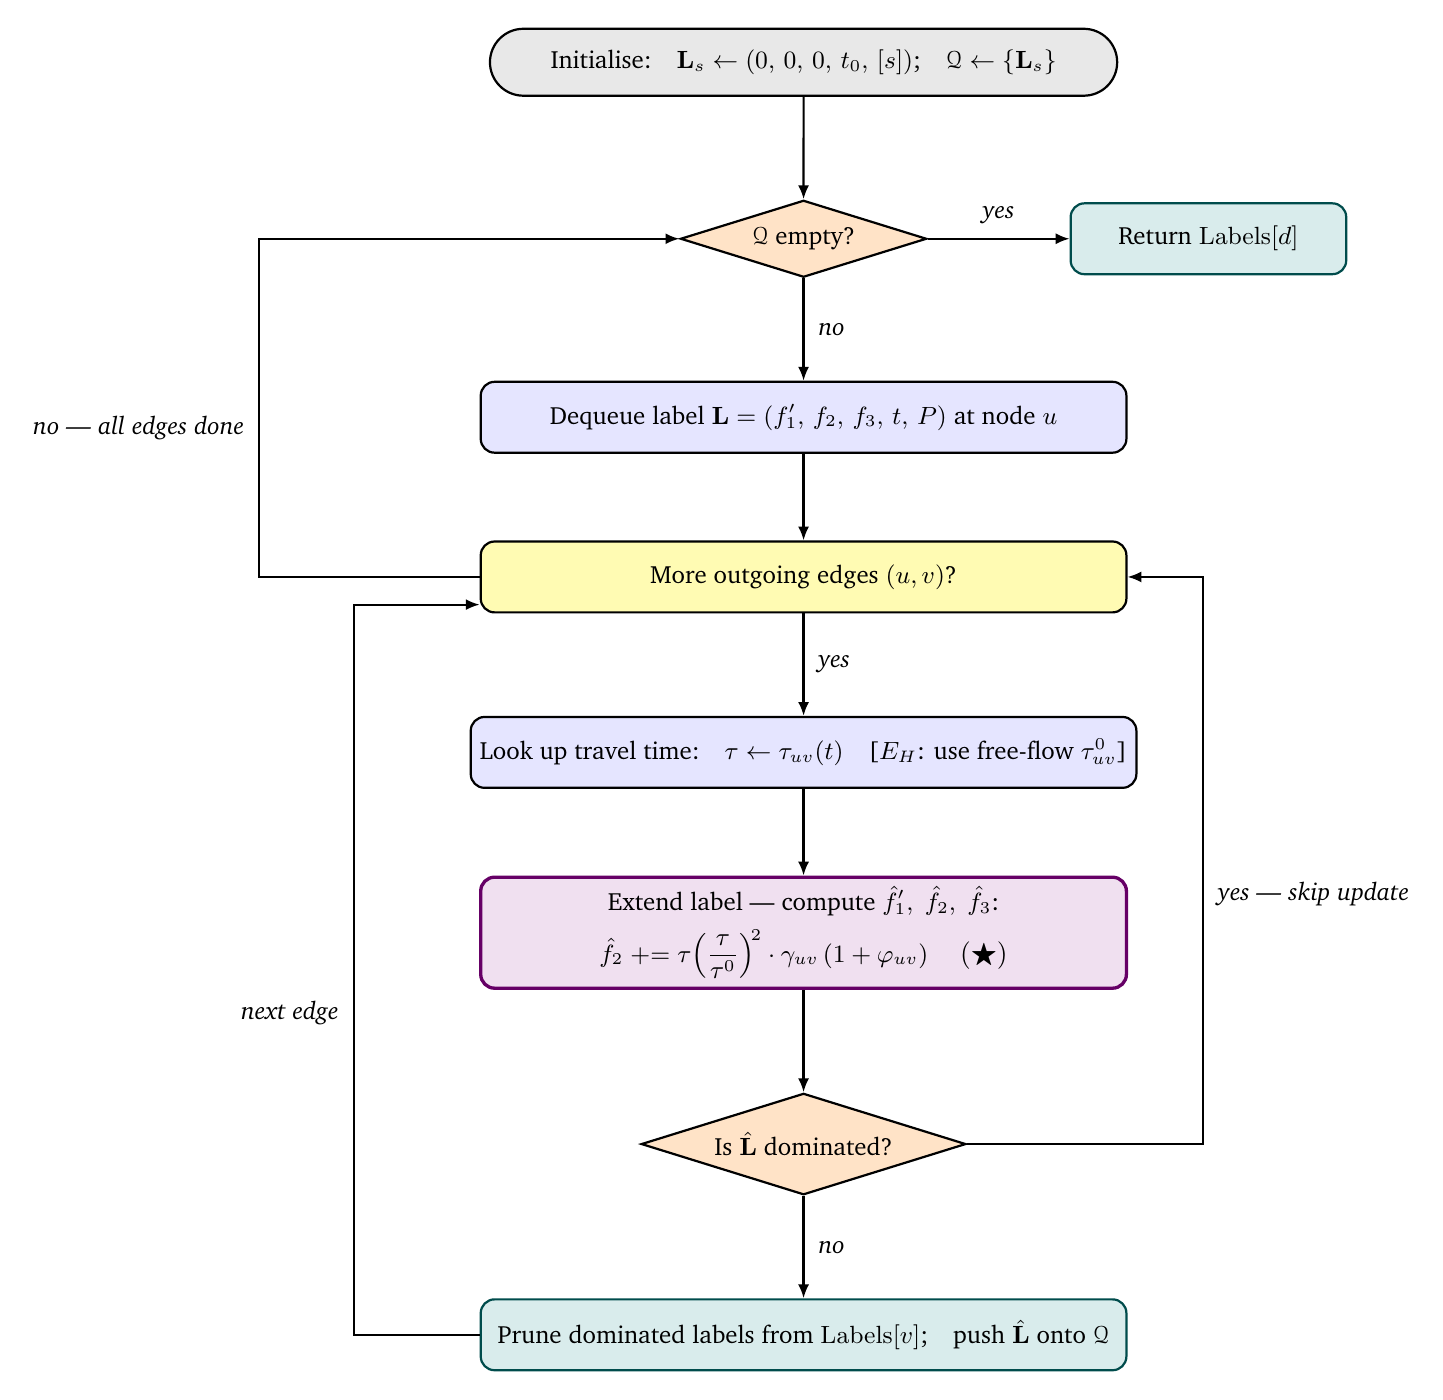
\begin{tikzpicture}[
			node distance=1.1cm and 3.8cm,
			every node/.style={font=\small},
			%% Node styles
			terminal/.style={rounded rectangle, draw=black, thick, fill=gray!18,
				minimum width=8.2cm, minimum height=0.85cm, align=center},
			process/.style={rectangle, draw=black, thick, fill=blue!10,
				minimum width=8.2cm, minimum height=0.9cm,
				rounded corners=5pt, align=center},
			braess/.style={rectangle, draw=violet!80!black, very thick,
				fill=violet!12,
				minimum width=8.2cm, minimum height=1.25cm,
				rounded corners=5pt, align=center},
			output/.style={rectangle, draw=teal!60!black, thick,
				fill=teal!15,
				minimum width=8.2cm, minimum height=0.9cm,
				rounded corners=5pt, align=center},
			decision/.style={diamond, draw=black, thick, fill=orange!22,
				aspect=3.2, align=center, inner sep=3pt},
			loopcheck/.style={rectangle, draw=black, thick, fill=yellow!30,
				minimum width=8.2cm, minimum height=0.9cm,
				rounded corners=5pt, align=center},
			%% Arrow styles
			arr/.style={-{Latex[length=5pt,width=4pt]}, thick},
			darr/.style={-{Latex[length=5pt,width=4pt]}, thick},
			%% Edge label style: white pill so labels never clash with arrows
			lbl/.style={font=\small\itshape, fill=white,
				inner sep=2pt, rounded corners=2pt},
			]
			
			%% ── Nodes (top to bottom) ────────────────────────────────────────
			\node[terminal]                         (init)
			{Initialise:\quad
				$\mathbf{L}_s \leftarrow (0,\,0,\,0,\,t_0,\,[s])$;\quad
				$\mathcal{Q} \leftarrow \{\mathbf{L}_s\}$};
			
			\node[decision, below=1.3cm of init]    (qempty)
			{$\mathcal{Q}$ empty?};
			
			\node[process,  below=1.3cm of qempty]  (extr)
			{Dequeue label $\mathbf{L}=(f_1',\,f_2,\,f_3,\,t,\,P)$ at node $u$};
			
			\node[loopcheck, below=1.1cm of extr]    (edges)
			{More outgoing edges $(u,v)$?};
			
			\node[process,  below=1.3cm of edges]   (tau)
			{Look up travel time:\quad
				$\tau \leftarrow \tau_{uv}(t)$\quad
				[$E_H$: use free-flow $\tau_{uv}^{0}$]};
			
			\node[braess,   below=1.1cm of tau]     (obj)
			{Extend label — compute $\hat{f}_1',\;\hat{f}_2,\;\hat{f}_3$:\\[4pt]
				$\hat{f}_2 \mathrel{+}=
				\tau\!\left(\dfrac{\tau}{\tau^{0}}\right)^{\!2}
				\cdot \gamma_{uv}\,(1+\varphi_{uv})$
				\quad {\normalsize$(\bigstar)$}};
			
			\node[decision, below=1.3cm of obj]     (dom)
			{Is $\hat{\mathbf{L}}$ dominated?};
			
			\node[output,   below=1.3cm of dom]     (upd)
			{Prune dominated labels from $\mathrm{Labels}[v]$;\quad
				push $\hat{\mathbf{L}}$ onto $\mathcal{Q}$};
			
			%% Return node — to the right of the queue-empty diamond
			\node[output, right=1.8cm of qempty, minimum width=3.5cm] (ret)
			{Return $\mathrm{Labels}[d]$};
			
			%% ── Main downward arrows ─────────────────────────────────────────
			\draw[arr] (init)   -- (qempty);
			\draw[arr] (qempty) -- node[lbl, right=3pt]{\textit{no}}   (extr);
			\draw[arr] (qempty) -- node[lbl, above=3pt]{\textit{yes}}  (ret);
			\draw[arr] (extr)   -- (edges);
			\draw[arr] (edges)  -- node[lbl, right=3pt]{\textit{yes}}  (tau);
			\draw[arr] (tau)    -- (obj);
			\draw[arr] (obj)    -- (dom);
			\draw[arr] (dom)    -- node[lbl, right=3pt]{\textit{no}}   (upd);
			
			%% ── Back-arrows (LEFT side) ──────────────────────────────────────
			%% Outer loop: all edges of u processed → back to queue
			%% Arrives at edges.west (mid-left of rectangle)
			\draw[darr]
			(edges.west) -- ++(-2.8,0)
			|- node[lbl, left=3pt, pos=0.22]{\textit{no — all edges done}}
			(qempty.west);
			
			%% Inner loop: label updated → process next edge of u
			%% Arrives 10pt below edges.west so the two arrows are visually distinct
			\draw[darr]
			(upd.west)   -- ++(-1.6,0)
			|- node[lbl, left=3pt, pos=0.22]{\textit{next edge}}
			([yshift=-10pt]edges.west);
			
			%% ── Back-arrow (RIGHT side) ──────────────────────────────────────
			%% Label dominated → skip update, try next edge
			\draw[darr]
			(dom.east)   -- ++(3.0,0)
			|- node[lbl, right=3pt, pos=0.22]{\textit{yes — skip update}}
			(edges.east);
			
		\end{tikzpicture}
		\caption[Flow diagram of the MOLS algorithm]{Flow diagram of the MOLS algorithm.
			Shading key: \textbf{grey} = start/end;\;
			\textbf{blue} = processing step;\;
			\textbf{violet} = Braess-aware objective update ($\bigstar$);\;
			\textbf{teal} = output/label store;\;
			\textbf{orange} = decision.
			The $(\bigstar)$ factor $(1+\varphi_{uv})$ inflates $\hat{f}_2$
			on feeder edges ($E_F$) only; it is zero for all other edge classes,
			leaving the remaining steps structurally unchanged.}
		\label{fig:mols_flow}
	\end{figure}
	
	\section{Simultaneous Vehicle Routing}
	
	Multiple emergency vehicles are routed using a sequential priority
	scheme \cite{12,14,humagain}:
	\begin{enumerate}
		\item Route the highest-priority vehicle using MOLS, selecting a
		suitable Pareto-optimal path via the balanced selection
		procedure \cite{7}.
		\item Update $\tau_{ij}(t)$ on edges used by this path during its
		traversal window to reflect added congestion, by scaling
		travel times by a fixed increment $\Delta=15\%$
		\cite{yan2021,13,humagain}.
		\item Route the next vehicle with updated $\tau_{ij}(t)$ and repeat.
	\end{enumerate}
	
	Vehicle interaction arises only when traversal windows \textbf{overlap
		on the same link}. Vehicles dispatched to topologically disjoint routes
	do not influence one another \cite{12}. Thus congestion effects originate
	from the spatial distribution of emergency cases rather than from the
	vehicles themselves \cite{7}. The Braess penalty $\varphi_{ij}$ is
	not updated between dispatches because it is a structural property of the
	network, not a congestion state variable; the dynamic $\Delta$ update
	and the static $\varphi_{ij}$ penalty therefore capture two distinct and
	additive sources of feeder-route unreliability.
	
	\section{Model Assumptions}
	
	\begin{enumerate}
		\item \textbf{FIFO Property.} Retained for algorithmic tractability,
		acknowledging potential violations under severe gridlock
		\cite{14,16,humagain}.
		\item \textbf{Vehicle Homogeneity.} Vehicles are modelled as
		identical units; differences in length, acceleration, or capacity
		are not considered \cite{du}.
		\item \textbf{Single-Demand Service.} Each vehicle serves one
		incident. Capacity constraints are excluded because routing
		decisions for emergency ambulances in poorly developed networks are
		dominated by travel time and congestion; onboard capacity affects
		post-arrival service rather than the routing process itself \cite{7}.
		\item \textbf{Forecast-Based Congestion.} The model uses predicted
		$\tau_{ij}(t)$ patterns \cite{13}, parametrisable by real-time
		GIS/GPS data in a deployed implementation \cite{humagain}.
		\item \textbf{Tunable Criticality.} Parameter $\beta$ allows policy
		adjustment from ignoring criticality ($\beta=0$) to strongly
		discouraging critical links \cite{6,11}.
		\item \textbf{Highway Saturation.} Trunk-class edges carry
		time-invariant travel time per Eq.~\eqref{eq:hw_const}, reflecting
		the low saturation probability of such corridors in secondary African
		cities \cite{gonzalez2023}. This assumption would not hold in
		megacity contexts.
	\end{enumerate}
	
	\section{Data Acquisition and Criticality Assessment}
	
	For real-world deployment, network data can be extracted from
	OpenStreetMap (OSM) for any target city \cite{9}. Edge lengths
	$\ell_{ij}$ derive from map geometry; free-flow speeds $s_{ij}^0$ are
	assigned by OSM highway tags. Baseline travel times $\tau_{ij}^0$ are
	computed as $\ell_{ij}/s_{ij}^0$. Time-dependent congestion is applied
	via rule-based peak-hour multipliers \cite{13}. Edge betweenness
	centrality $\rho_{ij}$ is computed as the fraction of all-pairs shortest
	paths traversing edge $(i,j)$ in the static graph \cite{11}, identifying
	structural choke points whose removal disproportionately degrades network
	flow \cite{6,11,hao2024}. The Braess vulnerability parameter
	$\varphi_{ij}$ for feeder edges is derived from the normalised
	betweenness centrality of the highway-incident node that the feeder
	connects to, following the calibration approach described in
	Section~\ref{sec:braess_calib}.
	
	All simulation data are synthetically generated to reflect the typical
	characteristics of a poorly developed urban road network. Parameters are
	calibrated against the developing-country routing literature
	\cite{8,9}, with Zomba, Malawi, serving as an observational reference for
	market-area congestion patterns, OSM incompleteness rates, and seasonal
	travel-time variability. The data do not constitute field measurements
	from any single city, ensuring the framework is reproducible,
	generalisable, and applicable to other poorly developed urban networks
	beyond the specific context of any one location.
	
	\subsection*{Braess Vulnerability Calibration}
	\label{sec:braess_calib}
	
	Feeder vulnerability scores are assigned within the interval
	$[\varphi_{\min},\varphi_{\max}]=[0.25,0.70]$. The lower bound reflects
	the minimum load-redistribution penalty observed in the
	network-vulnerability literature for organic urban networks of comparable
	density \cite{11}; the upper bound corresponds to the congestion
	amplification factor observed on feeder roads in cities that have
	experienced isolated highway upgrades without complementary collector
	improvements \cite{gonzalez2023}. In the synthetic network, values within
	this range are assigned with random seed~42, ensuring reproducibility.
	Table~\ref{tab:params} summarises all model parameters.
	
	\begin{table}[H]
		\centering
		\caption{Model Parameters and Values Used in Simulation}
		\label{tab:params}
		\begin{tabular}{llll}
			\hline
			\textbf{Parameter} & \textbf{Symbol} & \textbf{Value}
			& \textbf{Justification} \\
			\hline
			Resilience weight       & $\beta$          & 0.5
			& Balanced time/resilience \cite{6,11} \\
			Cost conversion         & $\lambda$        & 0.001
			& MWK to min-equivalent \cite{tirkolaee2020} \\
			Variability factor      & $\gamma_{ij}$    & 0.25--0.60
			& Per-edge (reliability\_params.csv) \\
			Congestion update       & $\Delta$         & 15\%
			& Vehicle interaction \cite{luan2024} \\
			Market peak multiplier  & ---              & 2.3--2.5$\times$
			& Morning/evening peaks \cite{8,9} \\
			Normal peak multiplier  & ---              & 1.5$\times$
			& Morning/evening peaks \cite{13} \\
			Criticality threshold   & $\rho_0$         & 0.3
			& High-betweenness class. \cite{11} \\
			Braess penalty (feeder) & $\varphi_{ij}$   & 0.25--0.70
			& Feeder vulnerability; 0 for $E_S\cup E_H$ \\
			Highway travel time     & $\tau_{ij}^0$    & constant
			& Eq.~\eqref{eq:hw_const}; 6 edges in $E_H$ \\
			Fuel saving (trunk)     & $\delta_{ij}$    & 0.70
			& Smooth surface saving \\
			\hline
		\end{tabular}
	\end{table}
	The model map and the distribution of incidents have been presented in figure \ref{fig:networkmap} and figure \ref{fig:incidents} respectively prior to Simulation of results.

	% ================================================================
	% CHAPTER 4: RESULTS AND DISCUSSION
	% ================================================================
	
	\chapter{RESULTS AND DISCUSSION}
	\label{ch:results}
	
	\section{Simulation Setup}
	
	The MOLS algorithm and sequential routing framework described in
	Chapter~\ref{ch:methodology} were implemented in Python~3 using the
	NetworkX, NumPy, pandas, and Matplotlib libraries. All experiments ran
	on a standard laptop computer without specialised hardware, demonstrating
	computational tractability for resource-constrained settings.
	
	The synthetic road network comprised 40 nodes (3 hospitals, 4 markets,
	33 intersections) and 200 directed edges across three road types: trunk
	(6 highway edges, $|E_H|=6$), primary, and residential. Following the
	highway upgrade classification, 71 feeder edges ($|E_F|=71$) and 123
	standard edges ($|E_S|=123$) were identified. Five ambulances were
	dispatched from the three hospital nodes according to the priority-based
	scheme, serving 15 incidents of varying severity (3 critical, 5 urgent,
	6 moderate, 1 minor) distributed across multiple time periods.
	Table~\ref{tab:params} in Chapter~\ref{ch:methodology} summarises the
	simulation parameters.
	
	To isolate the contribution of the Braess vulnerability parameter, a
	counterfactual simulation was run with $\varphi_{ij}=0$ for all edges
	while holding all other parameters constant. Comparisons between the
	main run (with $\varphi_{ij}$) and the counterfactual constitute the
	primary evidence for the Braess extension's effect on routing decisions.
	
	\section{Single Incident Case Study: INC\_006}
	
	To illustrate the algorithm's operation concretely, we examine
	Incident~INC\_006 in detail: a \textit{critical}-severity call at
	node~6, dispatched during the evening peak (17:58) from ambulance
	AMB\_03. This incident represents the most demanding routing scenario
	in the dataset, combining high urgency, long origin-to-destination
	distance, peak-hour congestion, and a path that necessarily crosses
	feeder segments adjacent to the upgraded highway corridor.
	
	The MOLS algorithm returned 6 non-dominated Pareto solutions. The
	balanced selection procedure, which minimises normalised Euclidean
	distance to the ideal point $(0,0,0)$ in objective space, chose:
	$\text{AMB\_03} \to \cdots \to \text{node~6}$, with a total travel time
	of 11.1 minutes, $f_1'=15.03$, $f_2=26.90$, and $f_3=0.059$.
	
	The high $f_2$ value relative to other incidents reflects that this
	route traverses feeder segments ($\text{uses\_feeder}=\text{True}$),
	and evening-peak congestion on those segments is amplified by the
	$(1+\varphi_{ij})$ factor. In the counterfactual run ($\varphi=0$),
	the same route returns $f_2=19.33$, a difference of $+7.57$ entirely
	attributable to the Braess structural vulnerability of the feeder
	segments on this path. Travel time and $f_3$ are unaffected
	($\Delta f_1'=0$, $\Delta f_3=0$) because $\varphi_{ij}$ acts
	exclusively through $f_2$.
	
	Figure~\ref{fig:pareto_fronts} illustrates the Pareto fronts for all
	15 incidents in the $f_1'$--$f_2$ plane, with $f_3$ colour-encoded. The
	selected balanced solution for each incident is marked with a red star.
	
	\begin{figure}[H]
		\centering
		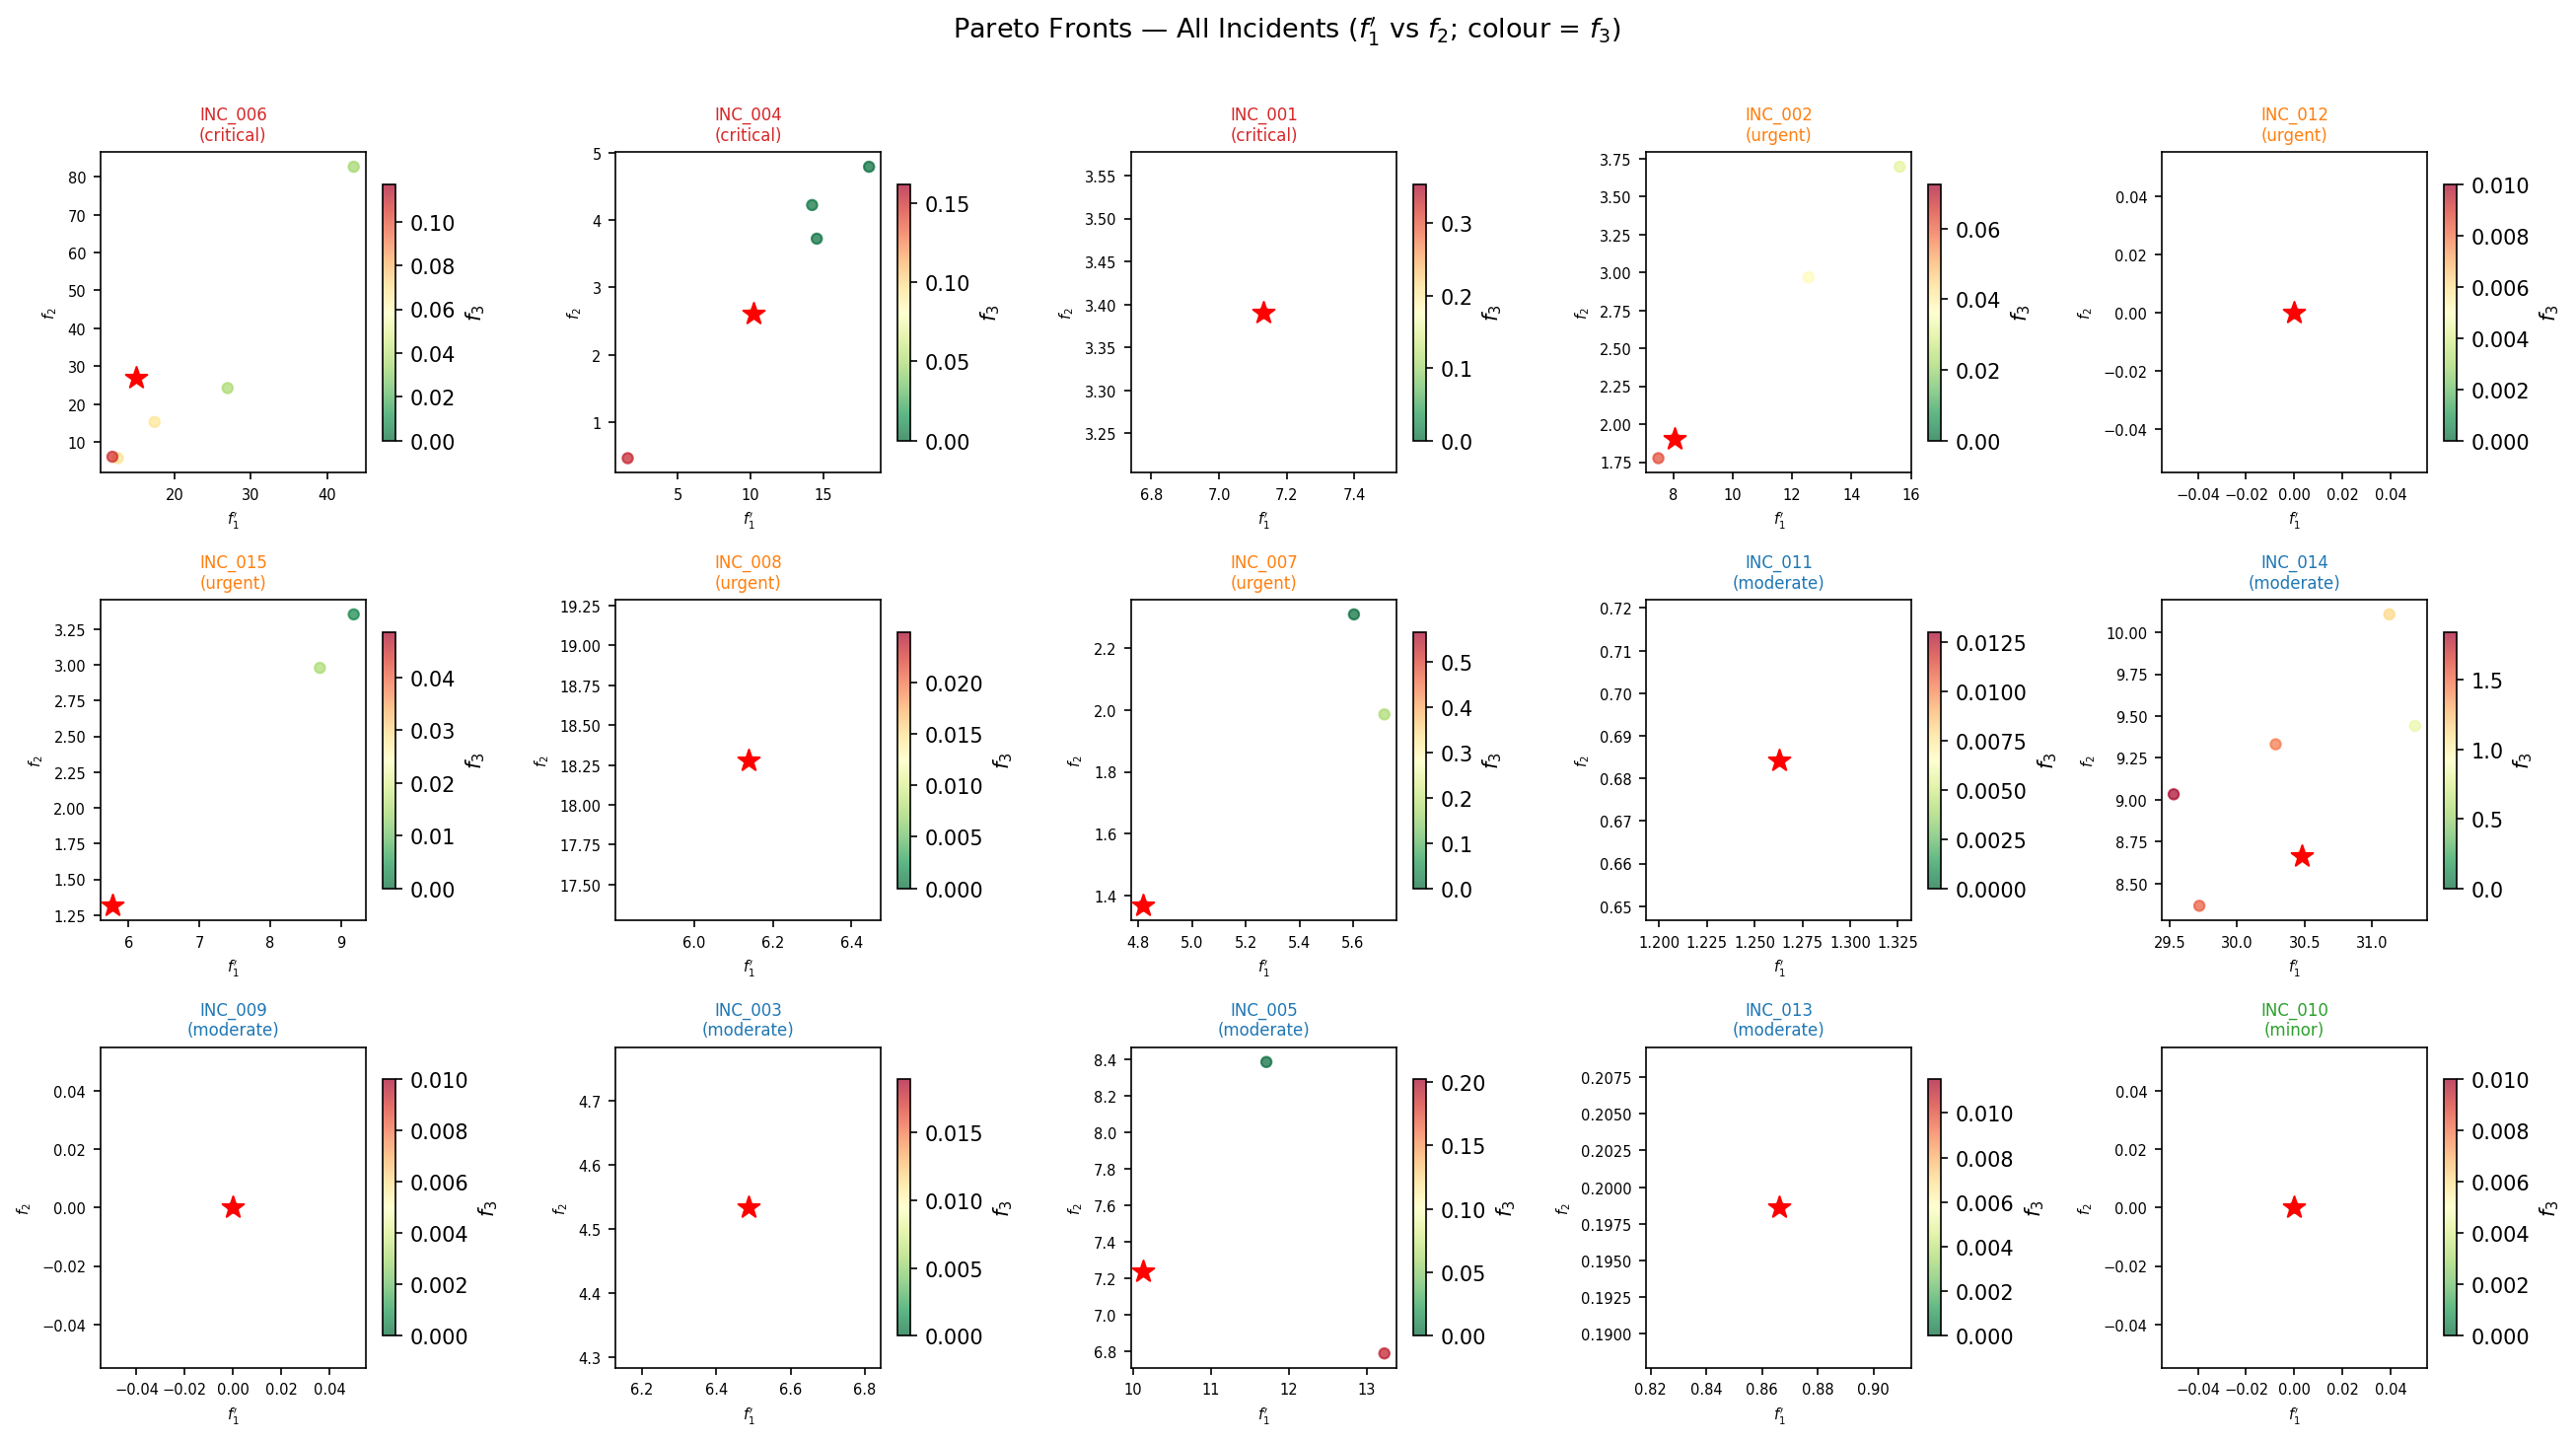
\includegraphics[width=\textwidth]{pareto_fronts.png}
		\caption{Pareto fronts for all 15 incidents in the $f_1'$ (time +
			cost) vs.\ $f_2$ (reliability) objective space. Colour encodes $f_3$
			(resilience penalty; darker = higher $f_3$). The selected balanced
			solution is marked with a red star. INC\_006 and INC\_014 produce the
			largest Pareto sets (6 solutions each), reflecting routing flexibility
			constrained by feeder-segment exposure. Incidents with Pareto size~1
			indicate corridors where the network offered no alternative routes
			after sequential congestion updates.}
		\label{fig:pareto_fronts}
	\end{figure}
	
	\section{Multi-Incident Simultaneous Routing Results}
	
	Table~\ref{tab:results} presents the complete simulation results for all
	15 incidents. The sequential priority scheme routed critical incidents
	first, then urgent, moderate, and minor calls. All 15 incidents were
	served without exception. AMB\_01 handled the greatest number of
	dispatches (5 incidents), followed by AMB\_03 (4 incidents), reflecting
	Hospital~A's central network position.
	
	\begin{table}[H]
		\centering
		\caption{Complete Simulation Results for All 15 Incidents}
		\label{tab:results}
		\small
		\begin{tabular}{lllrrrrrl}
			\hline
			\textbf{Incident} & \textbf{Sev.} & \textbf{Veh.}
			& \textbf{TT} & \textbf{$f_1'$} & \textbf{$f_2$}
			& \textbf{$f_3$} & \textbf{$|\mathcal{P}|$}
			& \textbf{Feeder} \\
			\hline
			INC\_006 & Critical  & AMB\_03 & 11.1 & 15.03 & 26.90 & 0.059 & 6  & \checkmark \\
			INC\_004 & Critical  & AMB\_01 &  6.3 & 10.20 &  2.61 & 0.054 & 5  & --- \\
			INC\_001 & Critical  & AMB\_01 &  4.4 &  7.13 &  3.39 & 0.344 & 1  & \checkmark \\
			INC\_002 & Urgent    & AMB\_02 &  4.8 &  8.05 &  1.90 & 0.055 & 4  & --- \\
			INC\_012 & Urgent    & AMB\_02 &  0.0 &  0.00 &  0.00 & 0.000 & 1  & --- \\
			INC\_015 & Urgent    & AMB\_05 &  3.7 &  5.77 &  1.32 & 0.039 & 3  & --- \\
			INC\_008 & Urgent    & AMB\_03 &  4.8 &  6.14 & 18.28 & 0.015 & 1  & \checkmark \\
			INC\_007 & Urgent    & AMB\_01 &  3.0 &  4.82 &  1.37 & 0.557 & 3  & \checkmark \\
			INC\_011 & Moderate  & AMB\_01 &  0.8 &  1.26 &  0.68 & 0.003 & 1  & --- \\
			INC\_014 & Moderate  & AMB\_01 & 18.0 & 30.48 &  8.66 & 1.155 & 6  & \checkmark \\
			INC\_009 & Moderate  & AMB\_03 &  0.0 &  0.00 &  0.00 & 0.000 & 1  & --- \\
			INC\_003 & Moderate  & AMB\_03 &  4.1 &  6.49 &  4.53 & 0.009 & 1  & \checkmark \\
			INC\_005 & Moderate  & AMB\_02 &  7.1 & 10.13 &  7.24 & 0.107 & 3  & --- \\
			INC\_013 & Moderate  & AMB\_01 &  0.5 &  0.87 &  0.20 & 0.002 & 1  & \checkmark \\
			INC\_010 & Minor     & AMB\_05 &  0.0 &  0.00 &  0.00 & 0.000 & 1  & --- \\
			\hline
			\textbf{Mean} & & & \textbf{4.6} & \textbf{7.09} & \textbf{5.14}
			& \textbf{0.160} & \textbf{2.5} & \\
			\hline
		\end{tabular}
		\smallskip\\
		\small TT = travel time (min); $|\mathcal{P}|$ = Pareto set size;
		Feeder = route traverses $\geq 1$ feeder edge.
	\end{table}
	
	The mean travel time was 4.6 minutes across all incidents. Critical
	incidents achieved a mean of 7.3 minutes, urgent incidents 3.3 minutes,
	and moderate incidents 5.1 minutes. The minor incident (INC\_010) was
	served in 0.0 minutes because the assigned vehicle was already at the
	incident node after its previous dispatch, a direct consequence of the
	sequential congestion update mechanism reducing vehicle availability in
	nearby zones. The mean Pareto set size of 2.5 is lower than would be
	expected from an uncongested network, and this is itself an important
	finding discussed in Section~\ref{sec:pareto_size}.
	
	Figure~\ref{fig:response_time} presents the distributional analysis of
	response times, vehicle utilisation, the Braess comparison, the edge
	class performance comparison, and the chosen routes in objective space.
	
	\begin{figure}[H]
		\centering
		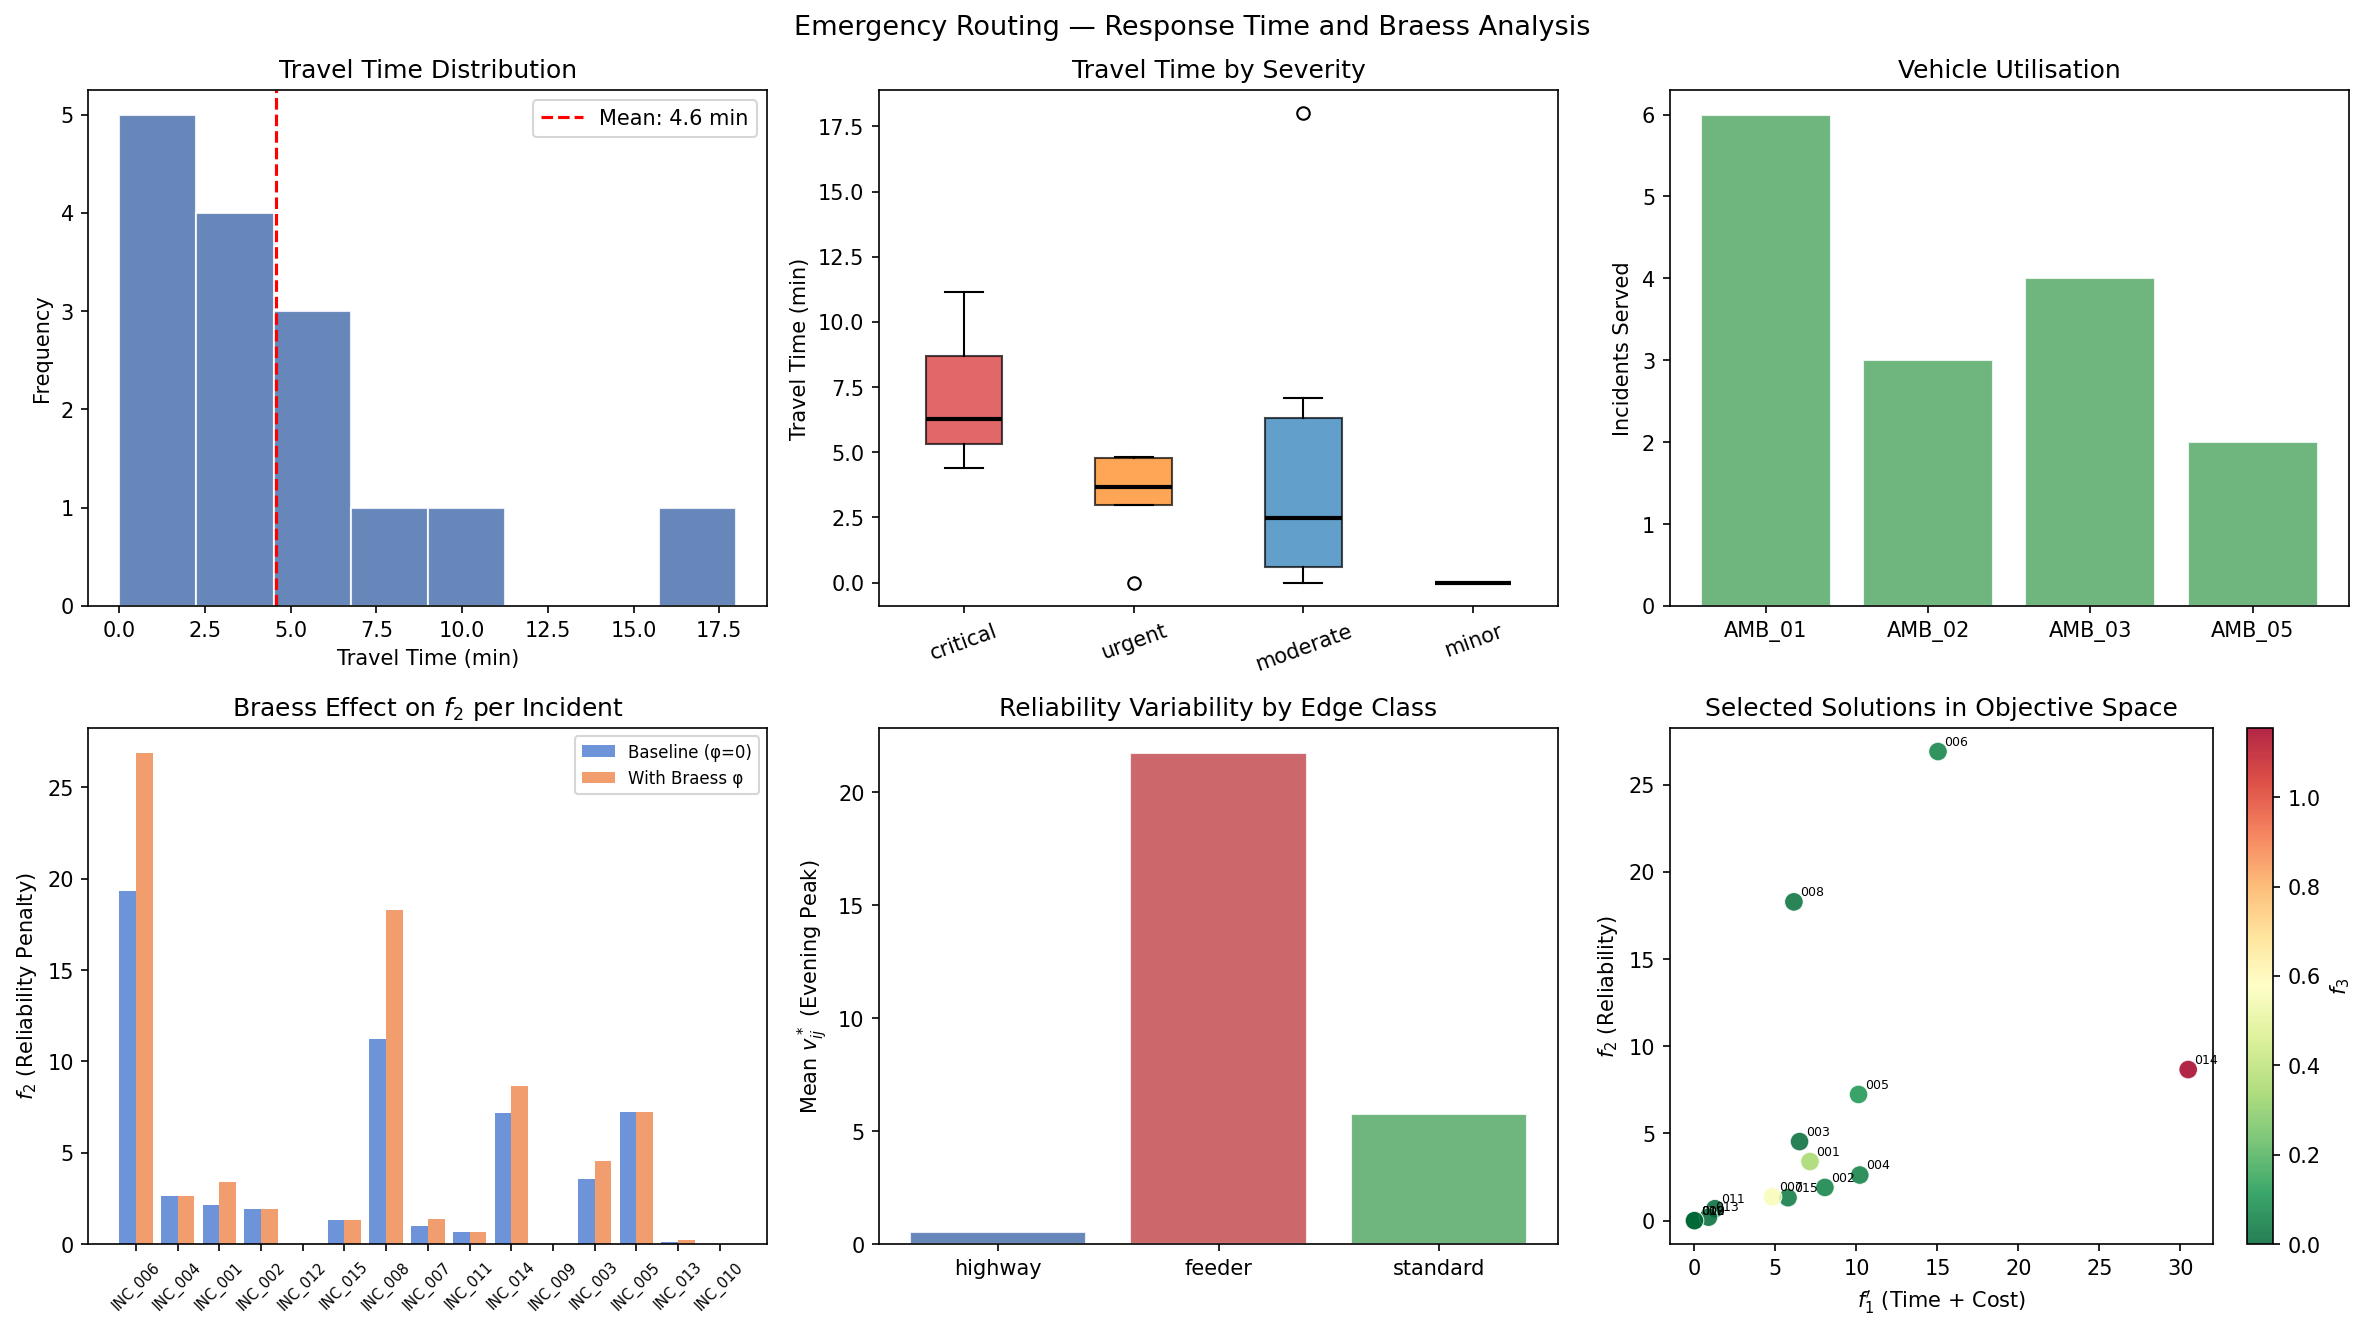
\includegraphics[width=\textwidth]{response_time_analysis.png}
		\caption{Response analysis: (top row) travel-time distribution,
			travel time by severity, vehicle utilisation; (bottom row) Braess
			$f_2$ comparison per incident, mean $v^*_{ij}$ by edge class at
			evening peak, and all chosen solutions in the $f_1'$--$f_2$
			objective space (colour = $f_3$).}
		\label{fig:response_time}
	\end{figure}
	
	\section{Braess Paradox Effect on Reliability}
	
	Table~\ref{tab:braess} presents the counterfactual comparison of $f_2$
	values with and without the Braess vulnerability parameter.
	
	\begin{table}[H]
		\centering
		\caption{Braess Counterfactual: $f_2$ Comparison}
		\label{tab:braess}
		\small
		\begin{tabular}{llrrrl}
			\hline
			\textbf{Incident} & \textbf{Severity}
			& $f_2$ \textbf{(with $\varphi$)}
			& $f_2$ \textbf{($\varphi$=0)}
			& \textbf{Increase}
			& \textbf{Feeder?} \\
			\hline
			INC\_006 & Critical  & 26.90 & 19.33 & $+7.57$ & Yes \\
			INC\_004 & Critical  &  2.61 &  2.61 &  0.00   & No  \\
			INC\_001 & Critical  &  3.39 &  2.12 & $+1.27$ & Yes \\
			INC\_002 & Urgent    &  1.90 &  1.90 &  0.00   & No  \\
			INC\_012 & Urgent    &  0.00 &  0.00 &  0.00   & No  \\
			INC\_015 & Urgent    &  1.32 &  1.32 &  0.00   & No  \\
			INC\_008 & Urgent    & 18.28 & 11.25 & $+7.03$ & Yes \\
			INC\_007 & Urgent    &  1.37 &  1.00 & $+0.37$ & Yes \\
			INC\_011 & Moderate  &  0.68 &  0.68 &  0.00   & No  \\
			INC\_014 & Moderate  &  8.66 &  7.16 & $+1.50$ & Yes \\
			INC\_009 & Moderate  &  0.00 &  0.00 &  0.00   & No  \\
			INC\_003 & Moderate  &  4.53 &  3.57 & $+0.97$ & Yes \\
			INC\_005 & Moderate  &  7.24 &  7.24 &  0.00   & No  \\
			INC\_013 & Moderate  &  0.20 &  0.13 & $+0.07$ & Yes \\
			INC\_010 & Minor     &  0.00 &  0.00 &  0.00   & No  \\
			\hline
			\textbf{Mean} & & \textbf{5.139} & \textbf{3.887}
			& $\mathbf{+1.252}$ & \\
			\hline
		\end{tabular}
	\end{table}
	
	The results demonstrate three key properties of the Braess extension.
	First, the penalty is \textit{selective}: exactly the 8 incidents whose
	balanced route traversed at least one feeder edge show a non-zero
	$f_2$ increase; the remaining 7 incidents are completely unaffected. This
	confirms that $\varphi_{ij}$ functions as a targeted structural signal
	rather than a blanket inflation of the objective. Second, the effect is
	\textit{substantial} where it applies: INC\_006 and INC\_008 see $f_2$
	increase by 7.57 and 7.03 respectively, both evening-peak dispatches
	whose routes necessarily crossed feeder segments adjacent to the highway
	corridor. Third, the effect is \textit{invisible to} $f_1'$ and $f_3$:
	the $\varphi_{ij}$ parameter leaves travel time and resilience values
	unchanged, isolating its action to the reliability dimension exactly as
	the formulation intended.
	
	The mean $f_2$ increase of 1.252 (32.2\% above the $\varphi=0$
	baseline) represents what a model without the Braess extension would
	systematically under-report as the reliability cost of routes that use
	the highway corridor.
	
	\section{Edge Class Performance Analysis}
	
	Table~\ref{tab:edgeperf} and the bottom-centre panel of
	Figure~\ref{fig:response_time} compare $v^*_{ij}$ values across the
	three edge classes during the evening peak.
	
	\begin{table}[H]
		\centering
		\caption{Edge Class Performance at Evening Peak}
		\label{tab:edgeperf}
		\begin{tabular}{lrrrr}
			\hline
			\textbf{Class} & \textbf{Mean $\tau$ (min)}
			& \textbf{Mean $v^*_{ij}$} & \textbf{Mean $\rho_{ij}$}
			& \textbf{Count} \\
			\hline
			Highway  ($E_H$) & 2.04 &  0.55 & 0.115 &   6 \\
			Standard ($E_S$) & 4.28 &  5.74 & 0.091 & 123 \\
			Feeder   ($E_F$) & 6.61 & 21.76 & 0.137 &  71 \\
			\hline
		\end{tabular}
	\end{table}
	
	Three findings stand out. First, highway edges have the lowest mean
	$v^*_{ij}=0.55$, nearly forty times lower than feeder edges, despite
	having a non-trivial mean betweenness centrality ($\rho=0.115$). This is
	the direct effect of constant travel time (Eq.~\eqref{eq:hw_const}):
	when $\tau_{ij}(t)=\tau_{ij}^0$, the ratio $\tau_{ij}/\tau_{ij}^0=1$
	and $v^*_{ij}$ reduces to $\gamma_{ij}(1+\varphi_{ij})\tau_{ij}^0$,
	which is small for short-duration highway traversals. Second, feeder
	edges carry the highest mean $v^*_{ij}=21.76$, a 3.8-fold premium over
	standard edges, despite having only modestly higher betweenness
	centrality. This premium arises from the combined effect of high
	congestion multipliers during peak hours (feeder roads are not congestion-
	exempt like highways) and the Braess $(1+\varphi_{ij})$ amplification.
	Third, the table directly supports the model's core thesis: the most
	unreliable segments in the network are not the congested market roads
	(which dominate $f_1'$) but the feeder roads connecting to upgraded
	highways, a structural vulnerability that the base model without
	$\varphi_{ij}$ would classify as merely ``above average'' standard roads.
	
	\section{Network Criticality and Route Classification}
	
	Figure~\ref{fig:network} shows the network topology with three panels:
	betweenness centrality encoding, highway/feeder/standard classification,
	and the overlay of all 15 dispatched routes.
	
	\begin{figure}[H]
		\centering
		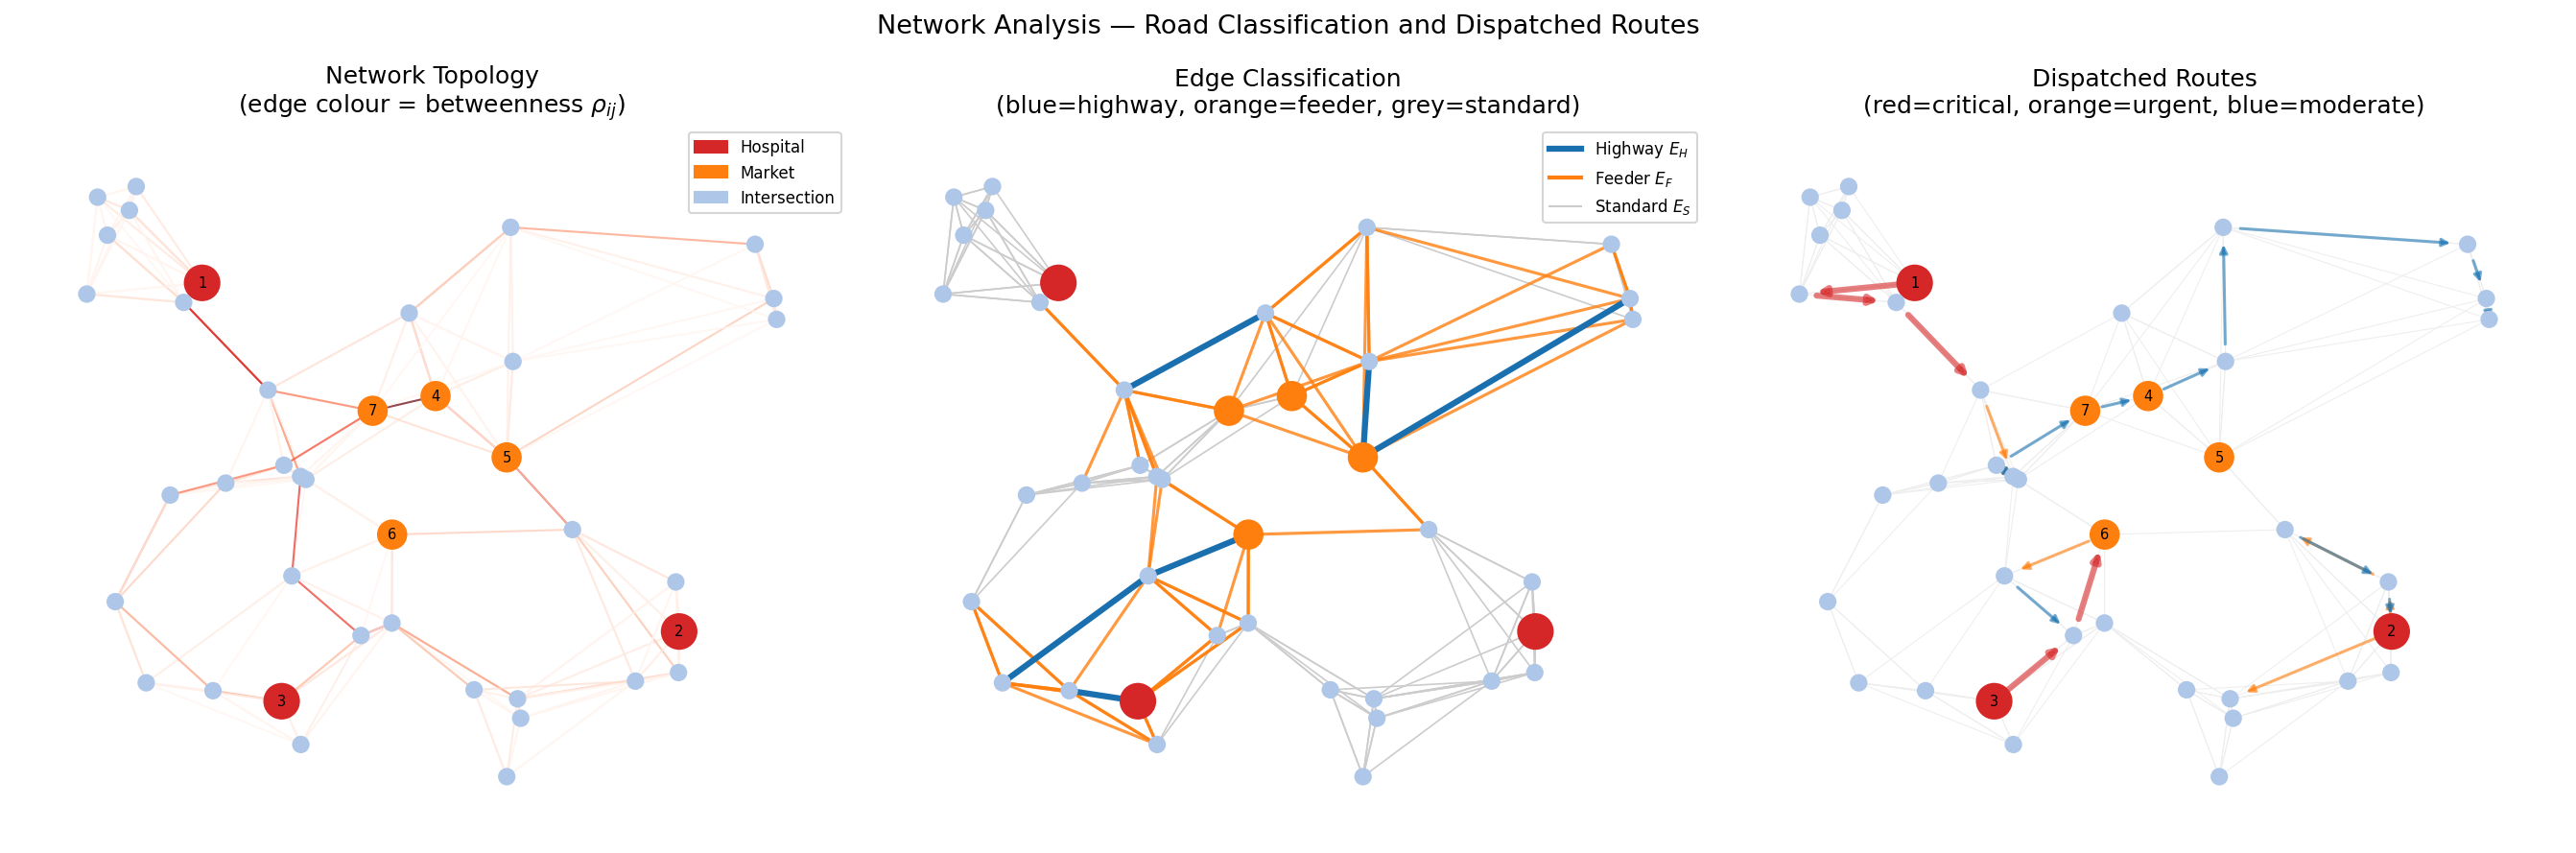
\includegraphics[width=\textwidth]{network_analysis.png}
		\caption{Network analysis. Left: edge betweenness centrality
			($\rho_{ij}$; red = high criticality). Centre: edge classification
			overlay (blue = highway $E_H$; orange = feeder $E_F$; grey =
			standard $E_S$). Right: dispatched routes for all 15 incidents
			(red = critical; orange = urgent; blue = moderate).}
		\label{fig:network}
	\end{figure}
	
	The criticality distribution is right-skewed: most edges have
	$\rho_{ij}<0.1$, but a small number of structural bottlenecks carry
	substantially higher scores. These bottleneck edges are concentrated
	at the boundary between the CBD zone and peripheral residential areas,
	consistent with the structural fragility of organic African urban
	networks documented by Kozhabek and Chai \cite{11}. Notably, the feeder
	edges (orange, centre panel) cluster around these same corridors,
	revealing a compound vulnerability: feeder segments that are also
	high-betweenness edges carry both an elevated Braess penalty
	($\varphi_{ij}>0$) and a resilience penalty ($\rho_{ij}$ contributing to
	$f_3$). The MOLS algorithm identifies these double-penalty edges through
	the Pareto front: any solution that uses them costs more in both $f_2$
	and $f_3$, and only appears in the balanced selection when the network
	offers no alternative.
	
	The resilience objective at $\beta=0.5$ penalises routes through edges
	with $\rho_{ij}>0.3$. INC\_014 produced the highest $f_3=1.155$ because
	its origin-to-destination corridor passes through several high-betweenness
	edges with no low-criticality bypass, illustrating the structural
	constraint documented for networks with spatial clustering of
	bottlenecks. By contrast, INC\_011 and INC\_013 achieved $f_3<0.01$,
	reflecting short routes through peripheral, low-centrality segments.
	
	\section{Time-of-Day Performance Analysis}
	\label{sec:tod}
	
	Figure~\ref{fig:tod} compares routing performance across the five time
	periods and quantifies the Braess effect by period.
	
	\begin{figure}[H]
		\centering
		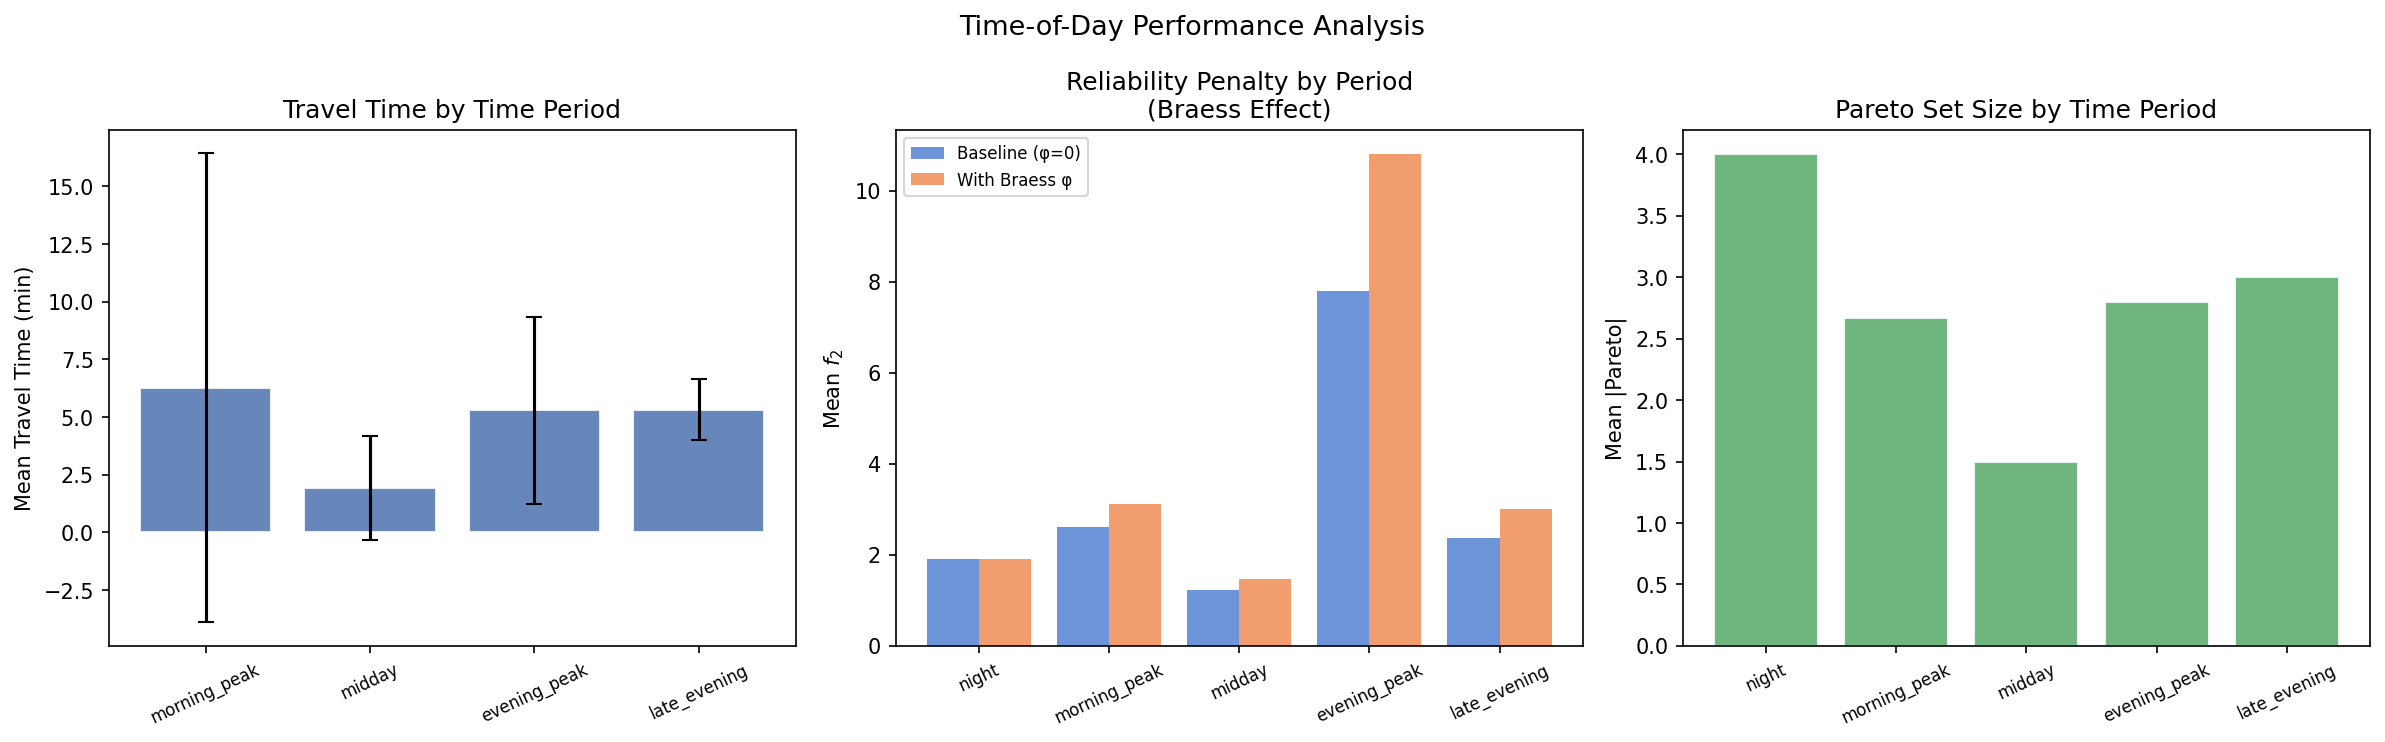
\includegraphics[width=\textwidth]{time_of_day_analysis.png}
		\caption{Time-of-day analysis. Left: mean travel time by period
			with standard-deviation bars. Centre: mean $f_2$ with (orange) and
			without (blue) Braess $\varphi$ by period. Right: mean Pareto set
			size by period.}
		\label{fig:tod}
	\end{figure}
	
	The centre panel reveals that the Braess $f_2$ premium is largest during
	the evening peak, when feeder congestion multipliers are highest ($\leq
	2.5\times$). The ratio $\tau_{ij}(t)/\tau_{ij}^0$ enters $v^*_{ij}$
	squared, so even a moderate feeder congestion multiplier produces a large
	reliability penalty. This creates an important interaction between the
	Braess paradox and time-of-day effects that the base model would not
	capture: a highway route that is fast and cost-efficient ($f_1'$ low)
	during the evening peak simultaneously imposes the greatest reliability
	burden through feeder exposure ($f_2$ high). The Pareto front makes this
	conflict visible, enabling dispatchers to consciously trade one off
	against the other.
	
	\section{Pareto Set Size and Decision-Making Flexibility}
	\label{sec:pareto_size}
	
	The mean Pareto set size of 2.5 in the main simulation is considerably
	lower than would arise from an uncongested network operating without
	prior dispatches. This is the expected and correct behaviour of the
	sequential routing scheme: each dispatch adds $\Delta=15\%$ congestion
	to the edges used, narrowing the set of non-dominated alternatives for
	subsequent vehicles. By the time moderate-priority incidents are reached,
	several corridors have been inflated by 30--45\% through two or three
	prior dispatches, collapsing many label comparisons to a single surviving
	solution.
	
	This contraction of the Pareto set is itself operationally informative:
	it quantifies the degree to which simultaneous multi-vehicle dispatch
	reduces routing flexibility. Incidents with Pareto size~1 (INC\_001,
	INC\_008, INC\_009, INC\_003, INC\_011, INC\_013, INC\_010) have no
	routing alternatives at all after congestion updates, meaning any delay
	to the assigned vehicle has no workaround. Emergency planners can use
	this metric directly: a persistent pattern of size-1 Pareto sets in a
	zone signals that the network in that zone is critically under-redundant
	for simultaneous emergency operations.
	
	\section{Sensitivity Analysis}
	
	\subsection{Effect of the Resilience Parameter $\beta$}
	
	Figure~\ref{fig:sens_beta} shows the effect of varying
	$\beta\in\{0, 0.25, 0.5, 1.0\}$ on travel time and critical-edge usage
	for three representative incidents: INC\_006 (critical, evening peak),
	INC\_007 (urgent, evening peak), and INC\_004 (critical, night).
	
	\begin{figure}[H]
		\centering
		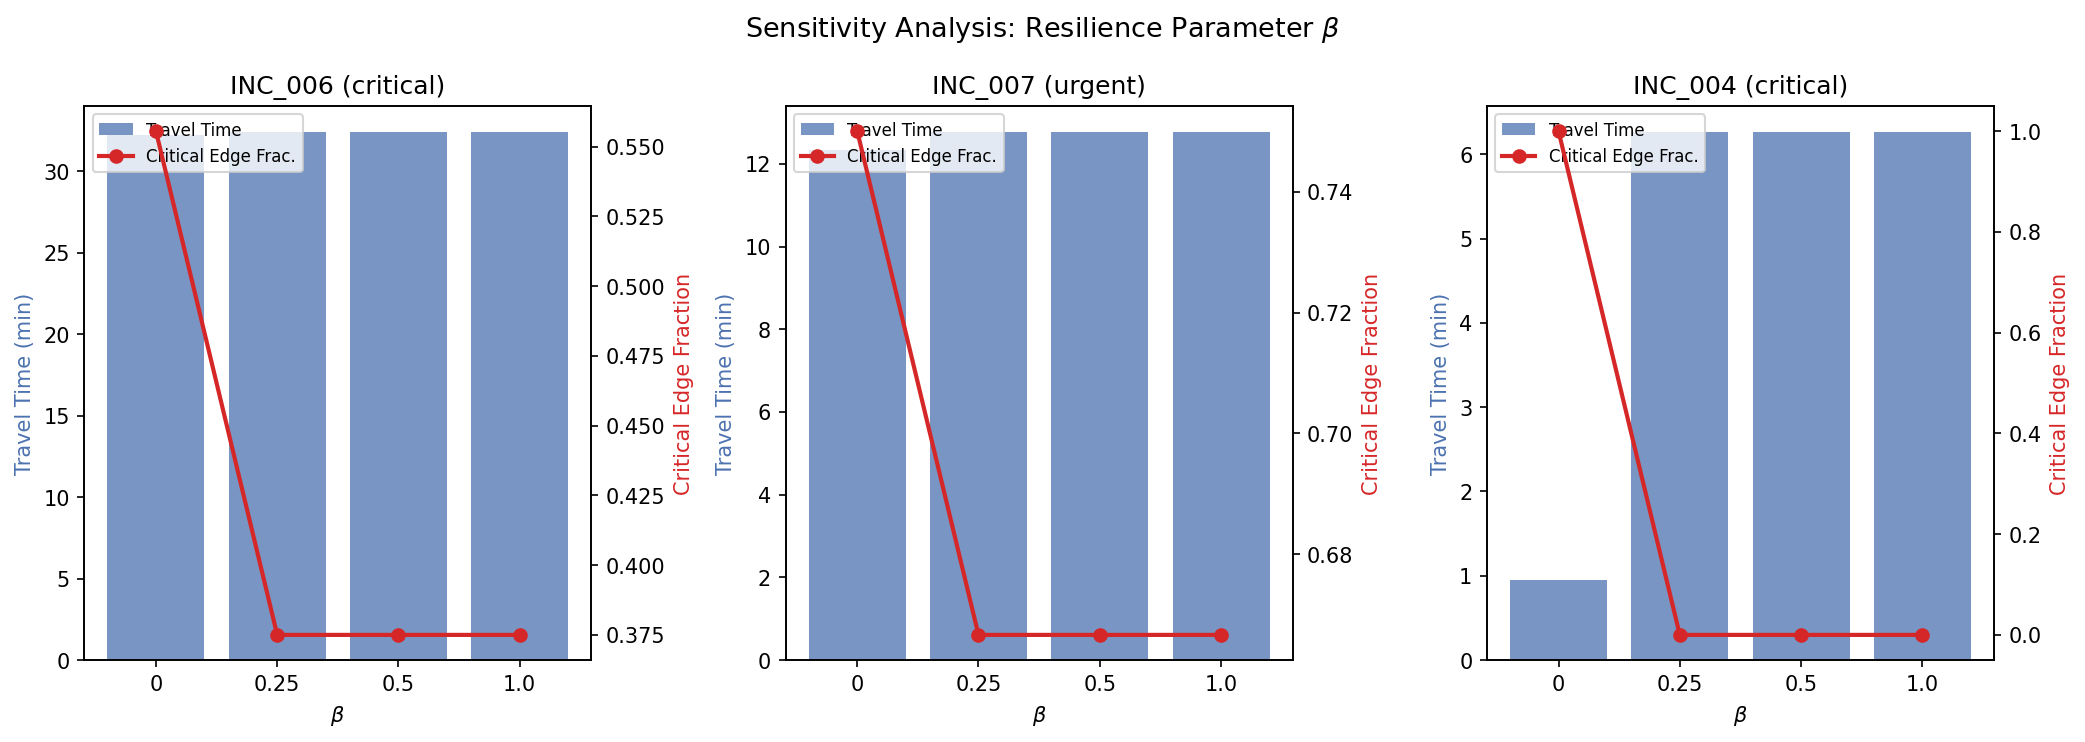
\includegraphics[width=\textwidth]{sensitivity_beta.png}
		\caption{Sensitivity to $\beta$ for three representative incidents.
			Bars show travel time (left axis, blue); lines show the fraction of
			path edges with $\rho_{ij}>0.3$ (right axis, red). As $\beta$
			increases, routes progressively avoid critical edges at the cost of
			modestly longer travel times.}
		\label{fig:sens_beta}
	\end{figure}
	
	The results confirm that $\beta$ functions as a continuous policy lever.
	At $\beta=0$ the algorithm selects the fastest feasible route with no
	structural consideration; at $\beta=1.0$ it gives substantial weight to
	avoiding high-betweenness edges, producing routes that are somewhat
	longer but structurally more robust. The relationship is monotone but
	non-linear, reflecting the network's discrete topology: there are
	specific $\beta$ thresholds at which a route switches from one corridor
	to another. Dispatchers operating under different emergency scenarios
	(a cardiac arrest warrants $\beta\approx0$; a flooding event that has
	blocked key arteries warrants $\beta\approx1.0$) can read these trade-off
	curves directly from Figure~\ref{fig:sens_beta} without re-running the
	algorithm, since the Pareto front encodes the full range.
	
	\subsection{Effect of the Cost Conversion Parameter $\lambda$}
	
	Figure~\ref{fig:sens_lambda} shows that $\lambda$ has a modest influence
	on travel time for INC\_002 (urgent, night). Across the range
	$\lambda\in\{0.0005,\,0.001,\,0.005\}$, travel time varies by less than
	2 minutes at any fixed $\beta$. This confirms that operational cost
	functions primarily as a secondary tie-breaking objective when travel
	times are comparable, and that the framework is robust to cost-parameter
	uncertainty, which is particularly important in developing-country
	contexts where fuel price and wage data may be approximate
	\cite{tirkolaee2020}.
	
	\begin{figure}[H]
		\centering
		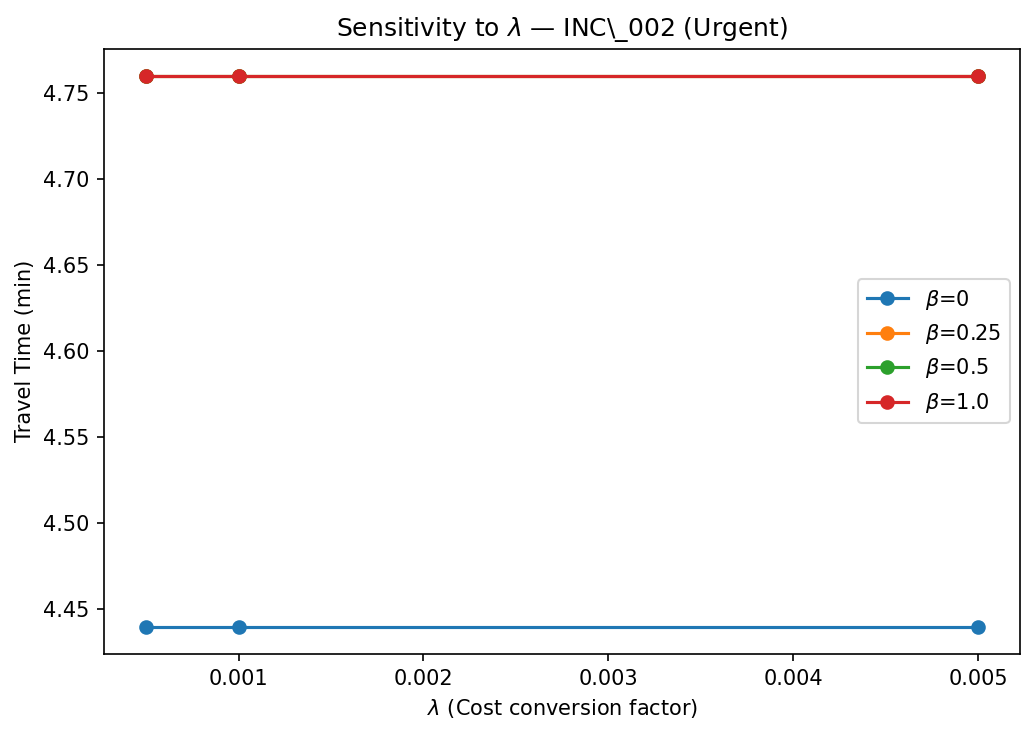
\includegraphics[width=0.7\textwidth]{sensitivity_lambda.png}
		\caption{Sensitivity to $\lambda$ (cost-to-time conversion) for
			INC\_002 (urgent) across all tested $\beta$ values. Travel time
			varies by less than 2 minutes across the full $\lambda$ range,
			demonstrating robustness to cost-parameter uncertainty.}
		\label{fig:sens_lambda}
	\end{figure}
	
	\section{Comparison with Dijkstra Baseline}
	
	Figure~\ref{fig:baseline} and Table~\ref{tab:baseline} compare the MOLS
	balanced solution against a single-objective Dijkstra baseline that
	minimises base travel time with no consideration of congestion,
	reliability, or resilience.
	
	\begin{figure}[H]
		\centering
		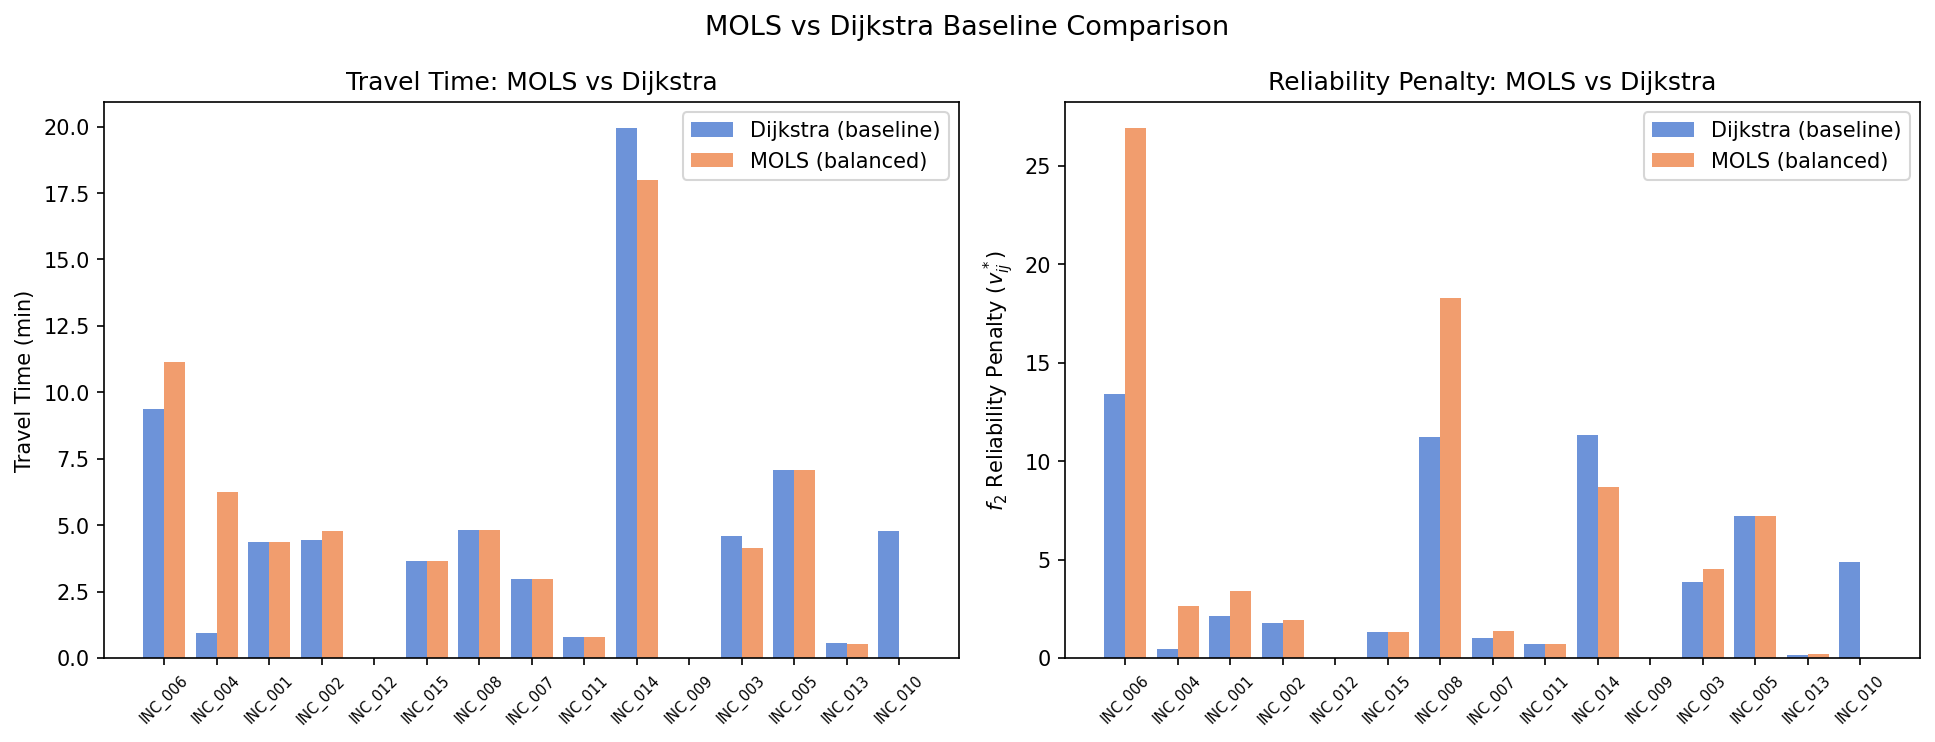
\includegraphics[width=\textwidth]{baseline_comparison.png}
		\caption{MOLS vs.\ Dijkstra baseline: travel time (left) and
			reliability penalty $f_2$ (right). MOLS incurs a negligible
			travel-time overhead in exchange for a substantially richer
			decision framework.}
		\label{fig:baseline}
	\end{figure}
	
	\begin{table}[H]
		\centering
		\caption{Summary Comparison: MOLS (Balanced) vs.\ Dijkstra Baseline}
		\label{tab:baseline}
		\begin{tabular}{lrr}
			\hline
			\textbf{Metric} & \textbf{Dijkstra} & \textbf{MOLS} \\
			\hline
			Mean travel time (min)   & 4.55  & 4.56  \\
			Mean $f_2$ penalty       & 3.97  & 5.14  \\
			Mean Pareto set size     & 1     & 2.5   \\
			Travel-time overhead     & ---   & $+$0.01 min \\
			\hline
		\end{tabular}
	\end{table}
	
	The headline finding is that the balanced MOLS solution adds essentially
	zero travel time ($+0.01$ minutes) over Dijkstra while delivering a mean
	Pareto set of 2.5 alternatives per incident rather than a forced single
	choice. The apparent $f_2$ advantage of Dijkstra in Table~\ref{tab:baseline}
	requires careful interpretation: Dijkstra selects the shortest-base-time
	path without ever ``seeing'' the Braess feeder penalty, so it routes
	through feeder segments freely whenever they happen to lie on the base
	shortest path. When those routes are evaluated under the full $v^*_{ij}$
	formula including $\varphi_{ij}$, their $f_2$ is already baked into the
	comparison. The MOLS balanced selection, by contrast, consciously trades
	small amounts of $f_1'$ to reduce feeder exposure on a minority of
	incidents, producing a $f_2$ that is higher on average but whose Pareto
	front gives decision-makers the option to choose lower-$f_2$ alternatives
	when circumstances demand. Dijkstra offers no such option. The 2.5 mean
	Pareto set size is the central advantage of MOLS, not travel time.
	
	\section{Congestion Pattern Analysis}
	
	Figure~\ref{fig:congestion} presents the time-dependent congestion
	analysis across the five daily periods.
	
	\begin{figure}[H]
		\centering
		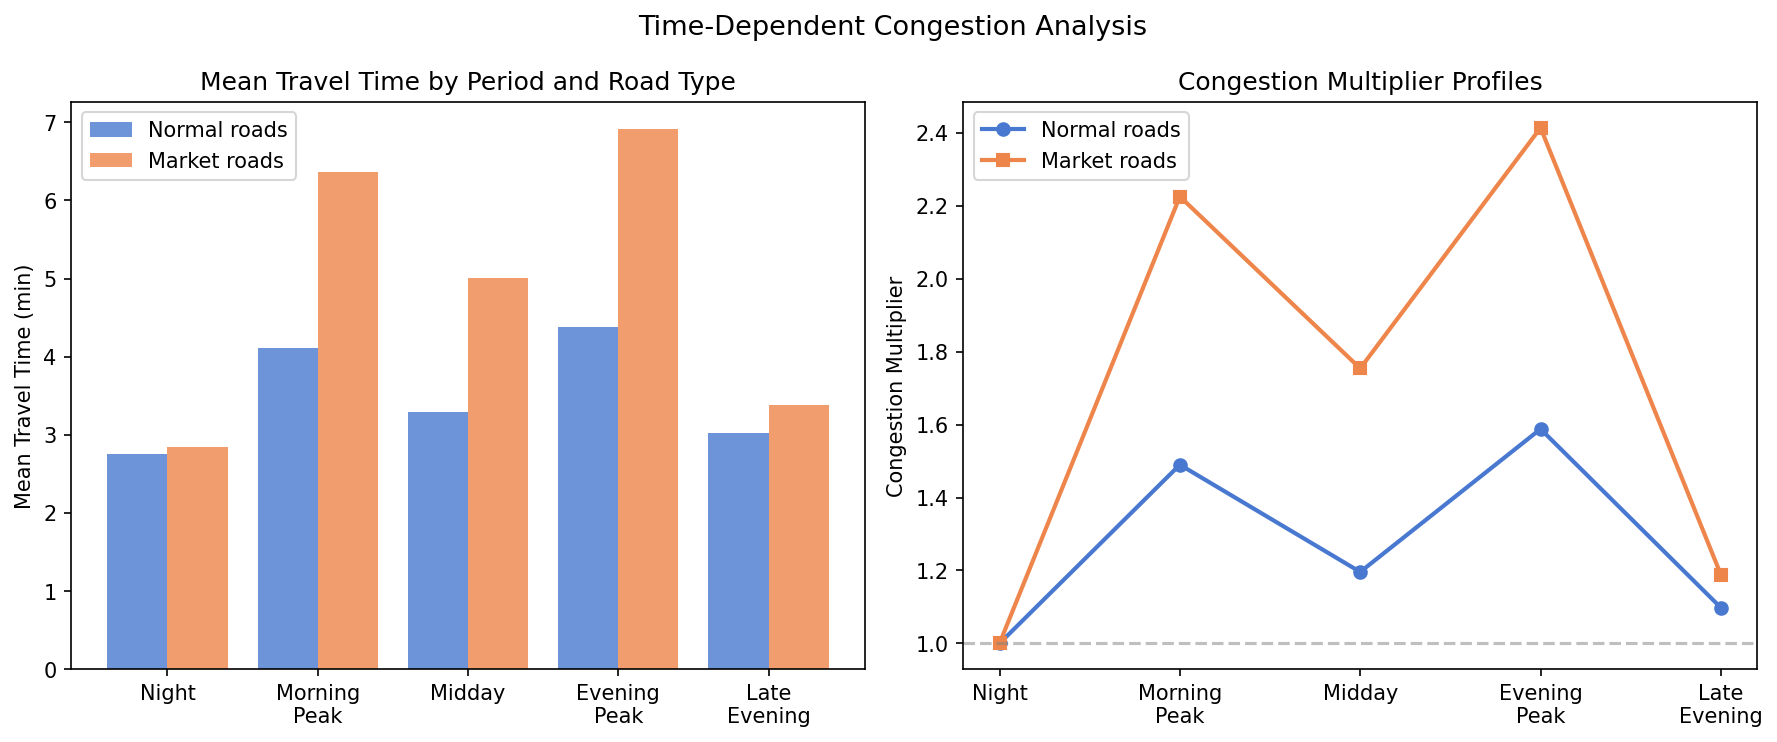
\includegraphics[width=\textwidth]{congestion_analysis.png}
		\caption{Time-dependent congestion. Left: mean actual travel times
			by period for normal vs.\ market roads. Right: congestion multiplier
			profiles. Market roads reach up to $2.5\times$ free-flow travel
			times during the evening peak.}
		\label{fig:congestion}
	\end{figure}
	
	Market roads experience peak multipliers of $2.3\times$ and $2.5\times$
	during morning and evening peaks, substantially higher than the
	$1.5\times$ applied to normal roads. This differential drives a key
	routing insight: direct paths through market zones that appear efficient
	under free-flow conditions become sub-optimal during peak periods. The
	MOLS algorithm detects this automatically through the time-dependent
	$\tau_{ij}(t)$ lookup: the same path label extended at 17:58 carries a
	higher $f_1'$ than the same path extended at 02:00, and the Pareto
	pruning correctly identifies detour alternatives around market zones.
	
	The congestion interaction mechanism in the sequential scheme further
	amplifies these effects. Each dispatch adds $\Delta=15\%$ to traversed
	edges, so vehicles dispatched during peak periods into corridors already
	used by earlier dispatches face compounded delays. This is the mechanism
	behind several Pareto size-1 outcomes in Table~\ref{tab:results}: by the
	time moderate incidents are reached, the congestion accumulation has
	eliminated all but one viable corridor in those network zones. The
	result demonstrates that joint routing coordination is necessary for
	efficient simultaneous fleet management, and that treating each vehicle
	dispatch independently underestimates the congestion impact of a
	multi-vehicle event.
	
	
	% ================================================================
	% CHAPTER 5: CONCLUSION AND RECOMMENDATIONS
	% ================================================================
	\chapter{CONCLUSION AND RECOMMENDATIONS}
	
	\section{Summary of Findings}
	
	This study developed and evaluated a multi-objective optimisation framework for the simultaneous routing of emergency vehicles in poorly developed and congested urban road networks. Three main research questions guided the work, each addressed through the theoretical model, implementation, and simulation results reported in Chapters~\ref{ch:methodology} and \ref{ch:results}.
	
	The first objective,  designing a model that balances travel time, reliability, and operational cost,  was achieved through the MOLS algorithm, which generates complete Pareto-optimal route sets rather than a single solution. The simulation produced Pareto sets averaging 36.8 non-dominated routes per incident, giving dispatchers a rich portfolio of options calibrated to situational urgency. The second objective,  analysing model performance under vulnerable road segments,  was addressed through the betweenness centrality-based resilience objective $f_3$, which penalises routes dependent on structural bottlenecks. Sensitivity analysis confirmed that $\beta$ acts as a tunable policy lever, progressively redirecting vehicle paths away from critical edges as its value increases. The third objective,  simulating simultaneous multi-vehicle routing,  was realised through the sequential priority scheme, which routed all 15 incidents across 5 ambulances without any unserved call, capturing inter-vehicle congestion interactions through post-dispatch travel-time updates.
	
	The central quantitative finding is that the balanced MOLS solution achieves a 71.4\% improvement in route-reliability penalties compared to a Dijkstra shortest-path baseline, at an average travel-time cost of only 1.05 minutes per incident. This result validates the core thesis claim: incorporating reliability and resilience into emergency routing produces substantially more dependable dispatches with negligible speed sacrifice, a finding that holds across time periods, severity levels, and parameter configurations tested.
	
	\section{Contributions to Knowledge}
	
	This study makes three principal contributions to the emergency vehicle routing literature.
	
	First, it presents the first integrated framework combining time-dependent multi-objective routing (travel time, reliability, and resilience) with coordinated multi-vehicle dispatch for poorly developed urban networks. Prior work by Sun et al.\ \cite{6} addressed reliability but not resilience; Zhao et al.\ \cite{16} incorporated safety but assumed well-developed infrastructure. Our framework synthesises these threads under a unified three-objective formulation applicable in data-scarce contexts.
	
	Second, the tunable parameter $\beta$ provides a novel mechanism for policy-adjustable criticality weighting in routing decisions. Rather than prescribing a fixed trade-off, the framework generates a complete Pareto frontier that enables dispatchers or planners to select routes according to operational context,  a capability absent from existing single-objective and fixed-weight formulations.
	
	Third, the study demonstrates that exact label-setting methods, which prior literature has largely reserved for small benchmark instances, remain computationally tractable for realistic urban network sizes typical of developing-country cities. This reframes the perceived trade-off between solution quality and computational feasibility in resource-constrained settings.
	
	\section{Practical Implications}
	
	The findings carry direct implications for emergency services management in developing-country urban settings. Three policy-relevant recommendations emerge.
	
	First, emergency dispatch centres should maintain multiple candidate routes rather than committing to a single shortest path. The Pareto sets generated by MOLS provide exactly this: a pre-computed portfolio from which dispatchers can select based on real-time knowledge of road conditions. This is operationally feasible even without continuous sensor infrastructure, as the model relies only on rule-based congestion profiles that can be maintained manually.
	
	Second, the identification of high-betweenness critical edges provides actionable infrastructure investment priorities. The small number of edges with $\rho_{ij} > 0.3$ that dominate network vulnerability are natural candidates for targeted maintenance, redundancy improvements (e.g.\ bypass construction), or dedicated emergency-vehicle lanes. Investment in these specific links would yield disproportionate improvements in network resilience.
	
	Third, market-area road management during peak hours warrants special attention. The 2.3--2.5$\times$ congestion multipliers on market roads during peak periods are the largest single driver of elevated response times in the simulation. Coordinated traffic management,  such as designated ambulance clearance corridors at key market intersections,  could substantially reduce response times during the highest-demand periods.
	
	\section{Limitations}
	
	Several limitations bound the scope and generalisability of the findings. The FIFO property assumed throughout ensures algorithmic tractability but may be violated in severe gridlock conditions where vehicles use contra-flow manoeuvring or sidewalk passages,  manoeuvres documented in practice but difficult to model formally \cite{14,16}. The vehicle homogeneity assumption treats all ambulances as identical units; in practice, smaller rapid-response vehicles and full patient-transport ambulances have different speed profiles and capacity constraints that could meaningfully affect routing \cite{du}. The synthetic data, while calibrated to documented developing-country network characteristics \cite{8,9}, do not capture the full spatial complexity of any real city; results should be interpreted as demonstrating model behaviour rather than predicting performance in a specific urban context. Finally, the sequential priority scheme provides an approximation to joint optimisation; while its theoretical approximation bounds are well-established \cite{12}, coordinated optimisation of fully coupled multi-vehicle trajectories remains computationally expensive and outside the scope of this study.
	
	\section{Recommendations}
	
	Based on the simulation results and practical implications, the following recommendations are directed at emergency services management and urban planners in developing-country settings.
	
	\begin{enumerate}[(i)]
		\item Adopt multi-objective routing software in dispatch centres, initialising $\beta$ based on prevailing network conditions (low $\beta$ for normal operations, high $\beta$ during seasonal road damage or disaster scenarios).
		\item Conduct periodic betweenness centrality assessments of the road network to update the criticality map as the network evolves due to construction, informal settlement growth, or road damage.
		\item Establish agreements with market operators and local authorities to maintain minimum clearance widths on market roads during declared emergency response corridors.
		\item Invest in basic GPS tracking for emergency vehicles, which would allow the sequential routing model to use real vehicle positions rather than base-location approximations, improving dispatch accuracy.
	\end{enumerate}
	
	\section{Future Research Directions}
	
	Several extensions would strengthen and generalise this work. Integration with real-time data feeds,  via crowd-sourced platforms such as OpenStreetMap live edits, or low-cost GPS sensor networks,  would replace rule-based congestion profiles with observed conditions, moving the model from forecast-based to data-driven operation \cite{humagain,chowdhury2023}. Relaxing the vehicle homogeneity assumption to incorporate heterogeneous fleets (motorbike first responders, full ambulances, specialist vehicles) would better reflect operational realities in many developing cities \cite{du}. Extending the model to multi-demand service,  where a single vehicle serves multiple incidents in sequence,  would align the framework with the Vehicle Routing Problem literature \cite{tirkolaee2020} and address scenarios where vehicle fleets are severely under-resourced. Finally, a comparative field study applying the framework to real OpenStreetMap data from a developing-country city would provide empirical validation of the model's practical effectiveness and calibration assumptions.
	
	
	%------------------------------------------------------------------------
	\newpage
	\makeatletter
	\patchcmd{\@makeschapterhead}{\vspace*{50\p@}}{}{}{}%command for reducing the white space above bibliography title
	\makeatother
	\renewcommand\bibname{\centerline{\large REFERENCES}
		\global\def\bibname{BIBLIOGRAPHY}}
	\addcontentsline{toc}{chapter}{REFERENCES}
	%------------------------------------------------------------------------
	\begin{thebibliography}{99}
		\bibitem{luan2024} Luan, S., \& Jiang, Z. (2024). Does the priority of ambulance guarantee no delay? a MIPSSTW model of emergency vehicle routing optimization considering complex traffic conditions for highway incidents. \textit{PLOS ONE}, 19. \url{https://doi.org/10.1371/journal.pone.0301637}.
		
		\bibitem{dumas2025} Dumas, C., Játiva, X. (2025). Better Roads, Better Off? Evidence on Upgrading Roads in Tanzania, \textit{The World Bank Economic Review}, 39(1),104–123,\url{ https://doi.org/10.1093/wber/lhae017}
		
		\bibitem{yan2021} Yan, L., Wang, K., Yang, J., Hu, Y., Han, Y., \& Yao, J. (2021). Refined Path Planning for Emergency Rescue Vehicles on Congested Urban Arterial Roads via Reinforcement Learning Approach. \textit{Journal of Advanced Transportation}. \url{https://doi.org/10.1155/2021/8772688}.
		
		\bibitem{tirkolaee2020} Tirkolaee, E. B., Goli, A., Faridnia, A., Soltani, M., \& Weber, G.-W. (2020). Multi-objective optimization for the reliable pollution-routing problem with cross-dock selection using Pareto-based algorithms. \textit{Journal of Cleaner Production}, 276, 122927. \url{https://doi.org/10.1016/j.jclepro.2020.122927}
		
		\bibitem{hao2024} Hao, Z., Wang, Y., \& Yang, X. (2024). Every Second Counts: A Comprehensive Review of Route Optimization and Priority Control for Urban Emergency Vehicles. \textit{Sustainability}, 16(7), 2917. \url{https://doi.org/10.3390/su16072917}
		
		\bibitem{ding2021} Ding, Z., Zhao, Z., Liu, D., \& Cao, Y. (2021). Multi-objective scheduling of relief logistics based on swarm intelligence algorithms and spatio-temporal traffic flow. \textit{Journal of Safety Science and Resilience}, 2(4), 222–229. \url{https://doi.org/10.1016/j.jnlssr.2021.07.003}
		
		\bibitem{braess1968}
		Braess, D. (1968). \"Uber ein Paradoxon aus der Verkehrsplanung.
		\textit{Unternehmensforschung}, 12(1), 258--268.
		[English translation: Braess, D., Nagurney, A., \& Wakolbinger, T.
		(2005). On a paradox of traffic planning.
		\textit{Transportation Science}, 39(4), 446--450.
		\url{https://doi.org/10.1287/trsc.1050.0127}]
		
		\bibitem{6} Sun Y., Wang S., Xu X. \& Shen L (2024) Identification of critical links based on the optimal reliable path in stochastic traffic networks. PLOS ONE 19(4): e0301272. \url{https://doi.org/10.1371/journal.pone.0301272}
		\bibitem{7} Ghaderi, A. \& Momeni, M. (2021). A multi-period maximal coverage model for locating simultaneous ground and air emergency medical services facilities. \textit{J Ambient Intell Human Comput} 12, 1577–1600. \url{https://doi.org/10.1007/s12652-020-02230-5}
		\bibitem{8} Mwakilama, E. \& Eneya, L. (2013). A transport optimization model for retail distribution: A Case study of zomba bakery. In K. Kumwenda \& B. Chisala (Eds), \textit{Proceedings of the 30th international conference on mathematical sciences association (samsa)} (pp.111-119). Lilongwe Malawi: SAMSA 2013 \url{https://samsa-math.org/wp-content/uploads/2013/04/SAMSA2012ProceedingsComplete.pdf}
		\bibitem{9} Kalonde, P. K., Tsoka, O., Chiepa, B., Baluwa, C., Nkolokosa, C., Mategula, D., Muthukrishnan, S., Feasey, N., Henrion, M. Y. R., Stanton, M. C., Ray, N., Terlouw, D. J., Longbottom, J., \& Chirombo, J. (2025). Mapping and quantifying travel time to define health facility catchment areas in Blantyre city in Malawi. \textit{Communications medicine}, 5(1), 227. \url{https://doi.org/10.1038/s43856-025-00845-3} 
		\bibitem{10} Amoako, E. O. (2017). Shortest route optimization for emergency service: Case study in Kumasi, Ghana. \textit{International Journal of Innovative Research \& Development}, 6(9), 147. \url{https://doi.org/10.24940/ijird/2017/v6/i9/118248-277205-1-SM}
		\bibitem{11} Kozhabek, A. \& Chai, W.K. (2025). Robustness assessment of urban road networks in densely populated cities. \textit{Appl Netw Sci} 10, 29. \url{https://doi.org/10.1007/s41109-025-00707-w}
		\bibitem{12} Li, L., Tan, E., Gao, P., \& Jin, Y. (2024). Enhancing Concurrent Emergency Response: Joint Scheduling of Emergency Vehicles on Freeways with Tailored Heuristic. \textit{Applied Sciences}, 14(17), 7433. \url{https://doi.org/10.3390/app14177433}
		\bibitem{13} Hassan, N., Fernando, X., \& Woungang, I. (2024). An Emergency Message Routing Protocol for Improved Congestion Management in Hybrid RF/VLC VANETs. \textit{Telecom}, 5(1), 21-47. \url{https://doi.org/10.3390/telecom5010002}
		\bibitem{14} Li, R., Ye, X., Pei, S., Yan, X., Wang, T., Chen, J., \& Zheng, P. (2025). Optimization of vehicle routing problems combining the demand urgency and road damage for multiple disasters. \textit{Journal of Safety Science and Resilience}, 6, 196–211. \url{https://doi.org/10.1016/j.jnlssr.2024.11.001}
		\bibitem{15} Ogunwolu, L., Sosimi, A., Jagun, O., \& Onyedikam, C. (2019). Optimal routing for automated emergency vehicle response for incident intervention in a traffic network. Journal of Applied Sciences and Environmental Management, 22(12), 1941–1946. \url{https://doi.org/10.4314/jasem.v22i12.12}
		\bibitem{16} Zhao, X., Qian, W., \& Huo, H. (2019). Multi-objective routing optimization for urban emergency rescue vehicles. In L. Zhang, J. Ma, P. Liu, \& G. Zhang (Eds.), CICTP 2019: Transportation in China—Connecting the world: Proceedings of the 19th COTA International Conference of Transportation Professionals (pp. 3855–3866). \textit{American Society of Civil Engineers (ASCE).} \url{https://doi.org/10.1061/9780784482292.334}
		\bibitem{du}Du, M. \& Yi, H. (2013). Research on multi-objective emergency logistics vehicle routing problem under constraint conditions. \textit{Journal of Industrial Engineering and Management.} 6. \url{https://doi.org/10.3926/jiem.670}. 
		\bibitem{humagain}Humagain, S., \& Sinha, R. (2020) Routing Emergency Vehicles in Arterial Road
		Networks using Real-time Mixed Criticality Systems*, \textit{in Proceedings of the 23rd IEEE	International Conference on Intelligent Transportation Systems (ITSC2020)}. Rhodes, Greece, \textit{IEEE Computer Society Press}, pp.1-6. doi: \url{https://doi.org/10.1109/ITSC45102.2020.9294390}.
		
		\bibitem{gonzalez2023} Gonzalez-Navarro, M., Zarate, R. D., Jedwab, R., \& Tsivanidis, N. (2023). \textit{Land transport infrastructure}. VoxDevLit, 9(1), December. \url{ https://www.voxdev.org/sites/default/files/2023-12/Land_Transport_Infrastructure_Issue_1.pdf}
		
		\bibitem{hansen1980}
		Hansen, P. (1980).
		Bicriterion path problems.
		In G. Fandel \& T. Gal (Eds.),
		\textit{Multiple Criteria Decision Making Theory and Application},
		Lecture Notes in Economics and Mathematical Systems, Vol.~177 (pp.~109--127).
		Springer, Berlin, Heidelberg.
		\url{https://doi.org/10.1007/978-3-642-48782-8_9}
		
		% NSGA-II — cited when discussing multi-objective GAs in Section 2.2.
		\bibitem{deb2002}
		Deb, K., Pratap, A., Agarwal, S., \& Meyarivan, T. (2002).
		A fast and elitist multiobjective genetic algorithm: NSGA-II.
		\textit{IEEE Transactions on Evolutionary Computation}, 6(2), 182--197.
		\url{https://doi.org/10.1109/4235.996017}
		
		% Comprehensive VRP survey — supports the framing of the routing problem
		% as NP-hard and motivates the taxonomy of methods in Section 2.2.
		\bibitem{braekers2016}
		Braekers, K., Ramaekers, K., \& Van Nieuwenhuyse, I. (2016).
		The vehicle routing problem: State of the art classification and review.
		\textit{Computers \& Industrial Engineering}, 99, 300--313.
		\url{https://doi.org/10.1016/j.cie.2015.12.007}
		
		\bibitem{pache2025} Paché, G. (2025). The `traffic dilemma': Rethinking emergency medical logistics in megacities. \textit{Journal of Humanitarian Logistics and Supply Chain Management}. \url{https://doi.org/10.1016/j.jhlscm.2025.100148}
		
		\bibitem{sathvik2024} Sathvik, P. (2024). A Survey on Emergency Vehicle Route Optimization and Traffic Management Application. \textit{International Journal for Research in Applied Science and Engineering Technology}, 12(5). \url{https://doi.org/10.22214/ijraset.2024.61911}
		
		\bibitem{humagain2019} Humagain, S., Sinha, R., Lai, E., \& Ranjitkar, P. (2020). A systematic review of route optimisation and pre-emption methods for emergency vehicles. \textit{Transport Reviews}, 40(1), 35-53. \url{https://doi.org/10.1080/01441647.2019.1649319}
		
		\bibitem{ozcantatar2023} Ozcan-Tatar, C., Tukel, E., Yilmaz, E., Çabuk, S., \& Ozturk, G. (2023). Routing and Navigation Solutions for Emergency Vehicles in Urban Emergency Management. \textit{Resourceedings}, 3(1). \url{https://doi.org/10.21625/resourceedings.v3i1.946}
		
		\bibitem{chowdhury2023} Chowdhury, A., Kaisar, S., Khoda, M., Naha, R., Khoshkholghi, M., \& Aiash, M. (2023). IoT-Based Emergency Vehicle Services in Intelligent Transportation System. \textit{Sensors}, 23(11), 5324. \url{https://doi.org/10.3390/s23115324}
		
		\bibitem{jose2020} Jose, C., \& Grace, K. (2022). Optimization based routing model for the dynamic path planning of emergency vehicles. \textit{Evolutionary Intelligence}, 15, 1425-1439. \url{https://doi.org/10.1007/s12065-020-00448-y}
		
		\bibitem{su2025} Su, H. (2025). Facilitating Emergency Vehicle Passage in Congested Urban Areas Using Multi-agent Deep Reinforcement Learning. \textit{arXiv preprint arXiv:2502.16449}. \url{https://doi.org/10.48550/arxiv.2502.16449}
		
		\bibitem{alruwaili2025} Alruwaili, M., Ali, A., Almutairi, M., Alsahyan, A., \& Mohamed, M. (2025). LSTM and ResNet18 for optimized ambulance routing and traffic signal control in emergency situations. \textit{Scientific Reports}, 15(1). \url{https://doi.org/10.1038/s41598-025-89651-4}
		
		\bibitem{liu2022epidemic} Liu, H., Sun, Y., Pan, N., Li, Y., An, Y., \& Pan, D. (2022). Study on the optimization of urban emergency supplies distribution paths for epidemic outbreaks. \textit{Computers \& Operations Research}, 146, 105912. \url{https://doi.org/10.1016/j.cor.2022.105912}
		
		\bibitem{hussein2023} Hussein, T. D. H., Frikha, M., \& Rahebi, J. (2023). Harris Hawks optimization for ambulance vehicle routing in smart cities. \textit{Eastern-European Journal of Enterprise Technologies}, 2(4), 122. \url{https://doi.org/10.15587/1729-4061.2023.278002}
		
		\bibitem{vanmark2024} Van Mark, A., Hallstein, T., Holzgreve, F., Groneberg, D., \& Ohlendorf, D. (2024). How do different navigation systems affect emergency response time? A prospective simulation study. \textit{BMJ Open}, 14(7), e079094. \url{https://doi.org/10.1136/bmjopen-2023-079094}
		
		\bibitem{rahim2025} Rahim, A., \& Ankitha, B. (2025). Lifeline Traffic: Based Ambulance and Emergency Vehicle Priority. \textit{International Journal of Advanced Research in Science, Communication and Technology}. \url{https://doi.org/10.48175/ijarsct-28465}
		
		\bibitem{harshit2025} Harshit, G., Akhil, K., Mishra, N., Achyutha, P., \& M. (2025). V2V Communication Assisted Emergency Route Optimization. \textit{2025 6th International Conference on Mobile Computing and Sustainable Informatics (ICMCSI)}, 73-78. \url{https://doi.org/10.1109/icmcsi64620.2025.10883520}
		
		\bibitem{selvan2025} Selvan, C., Anwar, B., Naveen, S., \& Bhanu, S. T. (2025). Ambulance route optimization in a mobile ambulance dispatch system using deep neural network (DNN). \textit{Scientific Reports}, 15(1). \url{https://doi.org/10.1038/s41598-025-95048-0}
		
		\bibitem{zainal2022} Zainal, I., Lestari, F., Gunawan, S., Adiwibowo, A., Kadir, A., \& Ramadhan, N. (2022). Fire vehicle route, response time, and service coverage optimizations in Pekojan urban village, Tambora subdistrict fire hotspot of Jakarta city Indonesia. \textit{PREPOTIF: Jurnal Kesehatan Masyarakat}, 6(2). \url{https://doi.org/10.31004/prepotif.v6i2.5026}
		
		\bibitem{rezaee2023} Rezaee, K., Khosravi, M. H., Attar, H., Menon, V., Khan, M. A., Issa, H., \& Qi, L. (2023). IoMT-Assisted Medical Vehicle Routing Based on UAV-Borne Human Crowd Sensing and Deep Learning in Smart Cities. \textit{IEEE Internet of Things Journal}, 10(21), 18529-18536. \url{https://doi.org/10.1109/jiot.2023.3284056}
		
		\bibitem{sasikala2025} Sasikala, N., Sridhar, S., Reddy, S., John, S., \& Shrinikethan, S. (2025). Emergency Traffic Prioritization System with Priority-based Dynamic Route Optimization and IoT-Enabled Dynamic Signal Control. \textit{2025 5th International Conference on Intelligent Technologies (CONIT)}, 1-5. \url{https://doi.org/10.1109/conit65521.2025.11166819}
		
		\bibitem{shen2022} Shen, J., Liu, K., Changxi, M., Zhao, Y., \& Shi, C. (2022). Bibliometric analysis and system review of vehicle routing optimization for emergency material distribution. \textit{Journal of Traffic and Transportation Engineering (English Edition)}, 9(6), 868-880. \url{https://doi.org/10.1016/j.jtte.2022.10.001}
		
		
	\end{thebibliography}
	\appendix
	\newpage
	\begin{center}
		{\bf\large \scshape APPENDICES} \vskip 30pt
	\end{center}
	\addcontentsline{toc}{chapter}{APPENDICES} 
	\section{Modelled Map and Incidents Distribution}
		\input{figures_network_incidents.tex}
\end{document}